%----------------------------------------------------------------------------------------
%	Metropolia Thesis LaTeX Template
%----------------------------------------------------------------------------------------
% License:
% This work is licensed under the Creative Commons Attribution 4.0 International License.
% To view a copy of this license, visit http://creativecommons.org/licenses/by/4.0/.
%
% However, this license apply to this template. As a template, it is supposed to be
% modified for your own needs (with your thesis content). For this reason, if you use
% this project as a template and not specifically distribute it as part of a another
% package/program, we grant the extra permission to freely copy and modify these files as
% you see fit and even to delete this copyright notice.
% In short, you are free to publish your thesis under whatever license you wish, even
% keep the all rights reserved to you.
%
% Authors:
% Panu Leppäniemi, Patrik Luoto, Mikaa Oni and Patrick Ausderau
%
% Credits:
% Panu Leppäniemi: abstract, def, cleaning,...
% Patrik Luoto: title page, abstract in Finnish, abbreviation, math,...
% Mikaa Oni: switch to biber biblatex
% Patrick Ausderau: initial version, style, table of content, bibliography, figure,
%                   appendix, table, source code listing,...
%
% Please:
% If you find mistakes, improve this template and alike, please contribute by sharing
% your improvements and/or send us your feedback there:
% https://github.com/panunu/metropolia-thesis-latex
% And of course, if you improve it, add yourself as an author.
%
% Compiler:
% Use XeLaTeX as a compiler. LuaLaTeX works too.
% Typical compilation:
% # minted require -shell-escape to run  external script.
% # -8bit avoid ^^I for tabs in minted.
% $ xelatex -shell-escape -8bit main
% # If any change in the bibliography
% $ biber main
% # If any change with the abbreviation or acronym
% $ makeglossaries main
% #Then compile again
% $ xelatex -shell-escape -8bit main
% #And if still some citation or label warnings, compile once more
% $ xelatex -shell-escape -8bit main

%----------------------------------------------------------------------------------------
%	THESIS INFO
%----------------------------------------------------------------------------------------

% All general information (main language, title, author (you), degree programme, major
% option, etc.)
% Edit the file chapters/0info.tex to change these information
\documentclass[12pt,a4paper,oneside,article]{memoir}%Do not touch this first line ;)

% Global information (title of your thesis, your name, degree programme, major, etc.)

\def\bilingual{yes}%For Finnish students, you must have 2 abstracts, one in English and one in your native language (Finnish or Swedish), so "yes", your thesis is bilingual.
%\def\bilingual{no}%For international student writing in English, only one language and one abstract.

\def\thesislang{finnish} %change this depending on the main language of the thesis.
%\def\thesislang{english} % "english" is the only other supported language currently. If someone has the swedish, please contribute!

\def\secondlang{english} %if the main language is Finnish (or Swedish), you must have 2 abstracts (one in Finnish (or Swedish) and one in English)
%\def\secondlang{finnish}
%If the main language is English and that you are native Finnish (or Swedish) speaker, you must have also abstract in your native language on top of the English one.

\author{Heikki Ketoharju} %your first name and last name

%\def\alaotsikko{Alaotsikko/Subtitle} %DISABLED, seems not to be an option with the 2018 template. If you really need it, uncomment and modify style/title.tex accordingly.

%License
%When publishing your thesis to theseus.fi, you can keep all rights reserved to you,
%or use one of the Creative Commons https://creativecommons.org/licenses/?lang=en
%This attribute will set the license in the metadata of the generated pdf.
%possible options (case sensitive):
%all (keep all rights reserved to yourself)
%by (Attribution)
%by-sa (Attribution-ShareAlike)
%by-nd (Attribution-NoDerivs)
%by-nc (Attribution-NonCommercial)
%by-nc-sa (Attribution-NonCommercial-ShareAlike)
%by-nc-nd (Attribution-NonCommercial-NoDerivs)
%Note that theseus do not accept dedication to public domain CC0
\def\thesiscopy{all}

%Finnish section, for title/abstract
\def\otsikko{Jaettua kieltä etsimässä – GraphQL-rajapinta tietomallin kohentelun
välineenä}
\def\tutkinto{Insinööri (AMK)} % change to your needs, e.g. "YAMK", etc.
\def\kohjelma{Tieto– ja viestintätekniikka}
\def\suuntautumis{Ohjelmistotuotanto}
\def\thesisfi{Insinöörityö}%was Opinnäytetyö
\def\ohjaajat{
Titteli Etunimi Sukunimi\newline
Titteli Etunimi Sukunimi
}
\def\tiivistelma{
Tämä on tiivistelmän ensimmäinen kappale. Tiivistelmän kappaleet loppuvat komentoon newline, jotta saadaan yksi tyhjä rivi aikaiseksi. \newline

Tämä on tiivistlemän toinen kappale.
}
\def\avainsanat{avainsana, avainsana}
\def\aihe{Lyhyt kuvaus opinnäytetyöstä. Max 255 merkkiä.}%for the pdf metadata/properties. If not used, empty it and also the \def\subject.

%English section, for title/abstract
\title{Your title here}
\def\metropoliadegree{Bachelor of Engineering} % change to your needs, e.g. "master", etc.
\def\metropoliadegreeprogramme{your degree programme (e.g. Information Technology)}
\def\metropoliaspecialisation{your major option (e.g. Mobile Solutions)}
\def\thesisen{Bachelor’s Thesis} % change to your need, e.g. master's
\def\metropoliainstructors{
First name Last name, Title (e.g.: Project Manager)\newline
First name Last name, Title (e.g.: Principal Lecturer)
}
\def\abstract{
Abstract content. To force newline between paragraph in the abstract, you must have both a empty line and the newline command. \newline

beginning of second paragraph\ldots
}
\def\metropoliakeywords{keyword, keyword}
\def\subject{short description of the thesis. Max 255 characters.}%for the pdf metadata/properties. If not used, empty it and also the \def\aihe.


%----------------------------------------------------------------------------------------
%	GLOBAL STYLES
%----------------------------------------------------------------------------------------

% If you need extra package, etc. modify the style/style.tex file.
% If you are using Windows OS, you will need to change default font to Arial in that
% style/style.tex file (or install Liberation Sans font to your system).
% If you are using MacOS or linux, make sure you have Liberation Sans font installed.
% Global style. Normally should not be edited.
% If you use windows OS, eventually change \setmainfont to Arial
% Check around commit https://github.com/panunu/metropolia-thesis-latex/commit/a0c15ac77bab1a52c59c517a18080938e57bf5ef
% to see how the font files were manually added (after downloading them: https://pagure.io/liberation-fonts/ )

%\usepackage[l2tabu, orthodox]{nag}%check for obsolete packages (with outdated nag package?)

%condition e.g. for adding or not space in TOC,...
\usepackage{etoolbox}
\ifdefstring{\bilingual}{yes}{
  \usepackage[\secondlang,\thesislang]{babel}% finnish (or swedish) and english
}{
  \usepackage[\thesislang]{babel}% english only
}
\usepackage{iflang}
\usepackage{amsmath}
\usepackage{amsfonts}%extra mathematical symbols
\usepackage{amssymb}
\usepackage{fontspec}
\usepackage{titlesec}
\usepackage{mathtools}%enhance the appearance of documents containing a lot of mathematics
\usepackage[amssymb]{SIunits}
\usepackage[version=3]{mhchem}
\usepackage{tikz} % mindmaps, flowcharts, piecharts, examples at http://www.texample.net/tikz/examples/
\usetikzlibrary{shapes.geometric, arrows}

\usepackage{ragged2e}
\IfLanguageName{finnish}{
  \RaggedRight%2021 template, align left and hyphennization for Finnish version
  \setlength{\RaggedRightRightskip}{0pt plus 1fil}%TODO: fix the Overfull/Underfull warnings when \RaggedRight (likely in title and abstact)
}{}
\makeatletter
  \let\@gnewline\@raggedtwoe@saved@gnewline% Restore original functionality of \newline
  \let\\\@raggedtwoe@savedcr% Restore original functionality of \\
\makeatother

%for compact list
\usepackage{enumitem}
%\usepackage{verbatim}%for block comment
%forcing single line spacing in bibliography
\DisemulatePackage{setspace}
\usepackage{setspace}
%\usepackage{eurosym}%euro symbol
%try to count
\usepackage{totcount}
%insert source code
%require -8bit -shell-escape in the xelatex compile command
%if compiling locally, consider options cachedir=minted,outputdir=~/.tex
\usepackage[newfloat]{minted}
\setminted{tabsize=2,linenos,breaklines,breaksymbolleft={\quad},baselinestretch=1}
\setmintedinline{breaklines,breakanywhere}
\usepackage[singlelinecheck=false]{caption}
%force the width of a table instead of column
\usepackage{tabularx}
\usepackage{booktabs} %why not booktabs? :3

\usepackage{csquotes}% avoid warning with babel

\usepackage{float} % For forced figure location with modifier H (\begin{figure}[H])
\usepackage{wrapfig}

% citep-macro for reference with period inside square brackets [1.]
\newcommand{\citep}[1]{
 \renewcommand\citeright{.]}
 \cite{#1}
 \renewcommand\citeright{]}
}

%set date format to D.M.YYYY
\def\pvm{\the\day.\the\month.\the\year}
%set date format to D Month YYYY
\usepackage[en,useregional=false]{datetime2}
\DTMsetup{datesep=.}
\DTMnewdatestyle{dMonthyyyy}
{%
  \renewcommand{\DTMdisplaydate}[4]{%
    \number##3 % day
    ~% separator
    \DTMenglishmonthname{##2}% month name
    ~% separator
    \number##1% year
  }%
  \renewcommand{\DTMDisplaydate}[4]{%
    \DTMdisplaydate{##4}{##3}{##2}{##1}%
  }%
}
\DTMsetdatestyle{dMonthyyyy}
\date{\today}

\newcommand\tn[1]{\textnormal{#1}} %use \tn instead of \textnormal
\newcommand\reaction[1]{\begin{equation}\ce{#1}\end{equation}} %\reaction{} for chemical reactions

%NORMAL TEXT
%all text, title, etc. in the same font: Arial
%NOTE: fontname is case-sensitive
\setmainfont[Scale=0.98]{Liberation Sans}
%line space
\linespread{1.46}
\AtBeginEnvironment{tabular}{\singlespacing}
%\doublespacing
%margin
%geometry moved after hyperref
\setlength{\parindent}{0pt} %first line of paragraph not indented
\setlength{\parskip}{16.5pt} %one empty line to separate paragraph
%list with small line space separation
\tightlists
\setlist[itemize]{before=\singlespacing,itemsep=6pt,leftmargin=63pt,labelsep=22pt,topsep=1.5pt,partopsep=0pt,after=\vspace{-22pt}\newline}
\setlist[enumerate]{before=\singlespacing,itemsep=6pt,leftmargin=63pt,labelsep=22pt,topsep=1.5pt,partopsep=0pt,after=\vspace{-22pt}\newline}

%IMAGE - FIGURE
%the figures should be placed in the "illustration" folder
\graphicspath{{illustration/}}
%figure number without chapter (1.1, 1.2, 2.1) to (1, 2, 3)
\counterwithout{figure}{chapter}
%border around images
\setlength\fboxsep{0pt}
\setlength\fboxrule{0.5pt}
%space after figure caption (and other float elements)
\setlength{\belowcaptionskip}{-7pt}
\setlength{\intextsep}{16.5pt}%space around floats
\AtBeginEnvironment{table}{\addvspace{16.5pt}}

%TABLE
\counterwithout{table}{chapter}

%SOURCE CODE
\newenvironment{code}{\captionsetup{type=listing}}{}
\IfLanguageName{finnish}{\SetupFloatingEnvironment{listing}{name=Koodiesimerkki}}{}%was Listaus
%\counterwithout{lstlisting}{chapter}
%moved after begin document, otherwise does not compile

%TOC
%change toc title
\IfLanguageName{finnish}{\addto{\captionsfinnish}{\renewcommand*{\contentsname}{Sisällys}}}{}
%remove dots
\renewcommand*{\cftdotsep}{\cftnodots}
%chapter title and page number not in bold
\renewcommand{\cftchapterfont}{\normalfont}
\renewcommand{\cftchapterpagefont}{\normalfont}
%sub section in toc
\setcounter{tocdepth}{2}
%subsection numbered
\setcounter{secnumdepth}{2}
\renewcommand{\tocheadstart}{\vspace*{-33.5pt}}
\renewcommand{\printtoctitle}[1]{\fontsize{13.5pt}{13.5pt}\bfseries #1\vspace*{-4pt}}
%\renewcommand{\aftertoctitle}{\vspace*{-22pt}\afterchaptertitle}
%spacing after a chapter in toc
\preto\section{%
  \ifnum\value{section}=0\addtocontents{toc}{\vskip11pt}\fi
}
%spacing after a section in toc
\renewcommand{\cftsectionaftersnumb}{\vspace*{-3pt}}
%spacing after a subsection in toc
\renewcommand{\cftsubsectionaftersnumb}{\vspace*{-1pt}}
%appendix in toc with "Appendix " + num
\IfLanguageName{finnish}{
  \renewcommand*{\cftappendixname}{Liite\space}
  \renewcommand{\appendixtocname}{Liitteet}
}{\renewcommand*{\cftappendixname}{Appendix\space}}
%appendix header
\IfLanguageName{finnish}{\def\appname{Liite\space}}{\def\appname{Appendix\space}}

%TITLES
%chapter title
%\clearforchapter{\clearpage}
\titleformat{\chapter}
{\fontsize{14pt}{14pt}\bfseries\linespread{1}}%\clearpage
{\thechapter}{.5cm}{}
\titlespacing*{\chapter}{0pt}{21.5pt}{.5pt}
\titleformat{\section}
{\fontsize{13.5pt}{13.5pt}\normalfont}
{\thesection}{.5cm}{}
\titlespacing*{\section}{0pt}{9pt}{0pt}
\titleformat{\subsection}
{\fontsize{12.7pt}{12.7pt}\normalfont}
{\thesubsection}{.5cm}{}
\titlespacing*{\subsection}{0pt}{11pt}{0pt}


%QUOTE
\renewenvironment{quote}
{\list{}{\rightmargin=0pt\leftmargin=2.2cm\topsep=-14pt}%
  \item\relax\singlespacing}%\fontsize{10pt}{10pt}
    {\vspace{8pt}\endlist}

%BIBLIOGRAPHY
%TODO: toggle for Harward v.s. Vancouver
\usepackage[
backend=biber,
bibencoding=utf8,%
citetracker=true,%
isbn=false,%
doi=false,%
url=true,%
usetranslator=true,%
bibstyle=ext-authoryear,%
citestyle=numeric-comp,%
sorting=none,%
sortcites=true,%
block=none,%
terseinits=false,%
giveninits=false,%
maxbibnames=99,%
]{biblatex}

\setlength{\bibitemsep}{11pt}
\setlength{\biblabelsep}{1cm}%with 1cm horizontal gap

\makeatletter
\RequireBibliographyStyle{numeric}
\makeatother

% set right format
\renewcommand*{\multicitedelim}{;\space}
\renewcommand*{\multinamedelim}{;\space}
\renewcommand*{\finalnamedelim}{~\&\space}
\DeclareFieldFormat{biblabeldate}{#1}
\DeclareDelimFormat[bib]{nameyeardelim}{\addperiod\space}
%\DeclareNameAlias{sortname}{last-first} % deprecated
\DeclareNameAlias{default}{family-given}
\DeclareFieldFormat{labelnumberwidth}{#1} % remove () from label number
\DeclareFieldFormat{title}{#1} % normal font for title
\DeclareFieldFormat{citetitle}{#1}
\DeclareFieldFormat{journaltitle}{#1} % remove underline
\DeclareFieldFormat*{url}{%
\ifentrytype{online}{\IfLanguageName{finnish}{Verkkoaineisto}{Online}\addperiod\space}{}%
\ifentrytype{video}{Video\addperiod\space}{}%
\textless\url{#1}\textgreater\addperiod
} % you can modify how to url looks here
%TODO: remove leading 0 for day and month for Finnish dates
\DeclareFieldFormat{urldate}{\space\bibstring{urlseen}\space#1} % remove () from date
%try set translation to biblio
\DefineBibliographyStrings{english}{%
    urlfrom = {available at},%
    urlseen = {Visited on},%
    fromenglish = {from English},%
    fromfinnish = {from Finnish},%
    fromgerman = {from German},%
    fromjapanese = {from Japanese},%
}
\DefineBibliographyStrings{finnish}{%
  %  urlfrom={Linkki: },%
    urlfrom = {},%
    urlseen = {Luettu},%
    fromjapanese = {japanista},%
    fromenglish = {englannista},%
    fromfinnish = {suomesta},%
    fromgerman = {saksasta},%
}
{
  %new cite command: "Vancouver Short"
  \DeclareCiteCommand{\citeVS}
    {\usebibmacro{prenote}}
    {\usebibmacro{author}, \usebibmacro{title}}
    {\multicitedelim}
    {\usebibmacro{postnote}}

  % new cite command: "Vancouver Short Collection" - necessary when referencing whole collections.
  \DeclareCiteCommand{\citeVSc}
    {\usebibmacro{prenote}}
    {\usebibmacro{editor}, \usebibmacro{title}}
    {\multicitedelim}
    {\usebibmacro{postnote}}
}

\addbibresource{biblio.bib}% for biblatex you need out \printbibliography too

%count the appendices (since the chapter counter is reset after \appendix).
%! require to complie 2 times
\regtotcounter{chapter}

% metadata (title, author, lang,...) for accessibility, etc.
\usepackage{hyperref}
\usepackage{hyperxmp}
\def\isolang{\IfLanguageName{finnish}{fi}{en}} %iso code (based on main language)
\ifdefstring{\thesiscopy}{all}{%
    \def\copyen{Copyright \textcopyright\ \the\year{}, \theauthor}
    \def\copyfi{Kaikki oikeudet pidätetään.  \textcopyright\ \the\year{}, \theauthor}
  }{%
    \usepackage[type={CC},modifier={\thesiscopy},version={4.0},]{doclicense}
    \def\copyen{\thetitle\ \textcopyright\ \the\year{} by \theauthor\ is licensed under \doclicenseLongNameRef}
    \def\copyfi{\otsikko\ \textcopyright\ \the\year{}, jonka tekijä on \theauthor, on lisensoitu \doclicenseLongNameRef}
}
\hypersetup{%
  pdfdisplaydoctitle,
  %breaklinks=true,%searching for overfull warnings
  pdfencoding=auto,
  bookmarksdepth=subsection,
  unicode=true,
  keeppdfinfo=true,
  pdflang={\isolang},
  pdfmetalang={\isolang},
  pdftitle={\IfLanguageName{finnish}{\otsikko}{\thetitle}},
  pdfkeywords={\IfLanguageName{finnish}{\avainsanat}{\metropoliakeywords}},
  pdfcopyright={\IfLanguageName{finnish}{\copyfi}{\copyen}},
  pdfsubject={\IfLanguageName{finnish}{\aihe}{\subject}},
}

\ifdefstring{\bilingual}{yes}{%metadata (title and copyright) in multiple language
  \XMPLangAlt{\IfLanguageName{finnish}{en}{fi}}{%
    pdftitle={\IfLanguageName{finnish}{\thetitle}{\otsikko}},
    pdfcopyright={\IfLanguageName{finnish}{\copyen}{\copyfi}},
    pdfsubject={\IfLanguageName{finnish}{\subject}{\aihe}},
  }
}{}
\urlstyle{same}

%moved after hyperred as can cause conflicts
\usepackage{pdfcomment}%try the alt text for graphics
\usepackage{accsupp}
\newcommand{\AltText}[2]{\BeginAccSupp{method=pdfstringdef,unicode,Alt={{#1}}}\pdftooltip{{#2}}{{#1}}\EndAccSupp{}}

\usepackage[top=2.5cm, bottom=3cm, left=4cm, right=2cm, nofoot]{geometry}

\usepackage{pgfplots} %simple plots etc
\pgfplotsset{compat=1.16}
\usepackage{pgfplotstable}

% Abbreviations, acronym and glossary, in case of bug, remove temporary the noredefwarn
\usepackage[acronym,toc,nonumberlist,section=chapter,noredefwarn]{glossaries}%xindy,%toc, ,nomain
\newglossarystyle{mystyle}{%
  \setglossarystyle{list}% base this style on the list style
  \renewcommand*{\glossentry}[2]{%
  \item[\glsentryitem{##1}%
    \glstarget{##1}{\glossentryname{##1}:}]
  \glossentrydesc{##1}\glspostdescription\space ##2}
}
\setglossarystyle{mystyle}

\renewcommand*{\glsclearpage}{}

% Normally, you do not need to modify the title style. It's content comes from the
% chapters/0info.tex file.
\input{style/title.tex}

%----------------------------------------------------------------------------------------
%	ABBREVIATION AND GLOSSARY
%----------------------------------------------------------------------------------------

% Add/edit all your acronyms, abbreviations, glossary entries, etc. definitions in
% chapters/0abbr.tex file.
% You can have as many as you wish. Only the ones you use in your text (inserted with
% \gls{} command) will print in the Glossary/Lyhenteet.
% Generate the glossary
\makeglossaries

% Acronyms, abbreviations, etc.

\newacronym{lamp}{LAMP}{LAMP (Linux, Apache, MySQL, PHP)}
\newacronym{orm}{ORM}{Object-relational mapper, oliot tietokantatauluiksi muuntava teknologia}
\newacronym{sql}{SQL}{Structured Query Language}
\newacronym{io}{I/O}{Input/Output}
\newacronym{ram}{RAM}{Random Access Memory}
\newacronym{php}{PHP}{Hypertext Preprocessor}
\newacronym{wysiwym}{WYSIWYM}{What You See Is What You Mean}
\newacronym{isbn}{ISBN}{International Standard Book Number}
\newacronym{url}{URL}{Uniform Resource Locator}
\newacronym{doi}{DOI}{Digital Object Identifier}


\newacronym{html}{HTML}{HyperText Markup Language}


% Glossary entries
\newglossaryentry{ddd}{
  name={Sovellusaluevetoinen suunnittelu},
  text={sovellusaluevetoinen suunnittelu},
  description={Menetelmä, jossa ohjelmistoa kehitetään läheisessä yhteistyössä sovellusalueen asiantuntijoiden kanssa. (myös: Liiketoimintavetoinen suunnittelu.) Engl. Domain Driven Design}
  }
\newglossaryentry{domain}{
  name={Sovellusalue},
  text={sovellusalue},
  description={Erityisala, jota sovellus käsittelee. Esimerkiksi pankkitoiminta tai vähittäiskauppa. myös: liiketoimintataso}
}

\newglossaryentry{crunching}{
  name={Tiedon rouhinta},
  text={tiedon rouhinta},
  description={Prosessi, jossa tunnistetaan sovellusalan erityiskäsitteitä ohjelmoijan ja sovellusalueen asiantuntijan välisen kommunikaation avulla. Engl. Knowledge crunghing}
  }
\newglossaryentry{dsl}{
  name={Täsmäkieli},
  text={täsmäkieli},
  description={Erityisalaan liittyvä formaali kieli. Esimerkiksi ohjelmointi- tai kuvauskieli. Engl. Domain-Specific language}
  }
\newglossaryentry{ubilang}{
  name={Kaikenkattava kieli},
  text={kaikenkattava kieli},
  description={Kokoelma käsitteitä ja sanastoa, joiden avulla ohjelmoijat ja sovellusalueen asiantuntijat keskustelevat kehitettävästä ohjelmistosta. Muotoutuu tiedon rouhintaprosessin tuloksena. Engl. Ubiquitous language}
  }
\newglossaryentry{domainmodel}{
  name={Sovellusaluemalli},
  text={sovellusaluemalli},
  description={Käsitteistä ja niiden välisistä suhteista koostuva, ohjelmakoodin muotoon kaapattava malli käsiteltävästä sovellusalueesta. Engl. Domain Model}
  }
\newglossaryentry{domainlayer}{
	name={Liiketoimintalogiikan taso},
	text={liiketoimintalogiikan taso},
	description={Ohjelmiston sisäinen osa, joka pitää sisällään liiketoimintaan liittyvän ohjelmalogiikan. Engl. Domain layer},
}
\newglossaryentry{entity}{
	name={Yksilötyyppi},
	text={yksilötyyppi},
	description={Ohjelmassa esiintyvä olio, jolla on identiteetti. Esimerkiksi yksittäinen asiakas tai lasku. Engl. Entity},
}
\newglossaryentry{deepermodel}{
  name={Syvempi malli},
  text={syvempi malli},
  description={Sovellusaluevetoisen suunnittelun myötä parantunut sovellusaluemalli. Syvempi malli tavoittaa aiempaa paremmin sovellusalan perimmäisen luonteen. Engl. Deeper Model}
}
\newglossaryentry{hakurakenne}{
  name={Assosiaatiotaulu},
  text={assosiaatiotaulu},
  description={Engl. Map. suom. myös {\em hakurakenne\/} ja {\em sanakirja\/}. Tietorakenne, joka sisältää joukon avain-arvo -pareja}
}

\newglossaryentry{rest}{
  name={REST},
  text={REST},
  description={Representational State Transfer. Arkkitehtoninen tyyli rajapintojen määrittelemiseen etenkin Web-sovelluksissa}
}

\newglossaryentry{graphql}{
  name={GraphQL},
  text={GraphQL},
  description={Facebookin kirjoittama kyselykieli, joka esittää manipuloitavan datan olioverkkona}
}

\newglossaryentry{http}{
  name={HTTP},
  text={HTTP},
  description={Hypertext Transfer Protocol. Webin perusprotokolla, jota käytetään hypertekstidokumenttien siirtoon}
}

\newglossaryentry{verkko}{
  name={Verkko},
  text={verkko},
  description={Tietorakenne, joka koostuu solmuista ja kaarista}
}

\newglossaryentry{domainexpert}{
  name={Alan asiantuntija},
  text={alan asiantuntija},
  description={Sovellusalueen esimerkiksi työnsä puolesta hyvin tunteva henkilö}
}

\newglossaryentry{kulkusuunta}{
  name={Kulkusuunta},
  text={kulkusuunta},
  description={Olioita yhdistävän kytköksen suunta}
}

\newglossaryentry{puhdasfunktio}{
  name={Puhdas funktio},
  text={puhdas funktio},
  description={Funktio, jonka palauttama tulos riippuu vain sen saamien parametrien arvoista. Puhdas funktio ei aiheuta sivuvaikutuksia esimerkiksi tulostamalla ruudulle tai tallentamalla tiedostoon}
}

\newglossaryentry{tyyppi}{
  name={Tyyppi},
  text={tyyppi},
  description={Lausekkeeseen sidottu määritys lausekkeen palauttaman arvon tietotyypistä. Esimerkiksi kokonaisluku tai merkkijono}
}

\newglossaryentry{aggregate}{
  name=Aggregaatti,
  text=aggregaatti,
  description={Useiden olioiden kokoelma, jolla on yksi juuriolio. Käsitellään ohjelmalogiikassa yhtenä kokonaisuutena.}
}
\newglossaryentry{repository}{
  name=Repositorio,
  text=repositorio,
  description=Rajapinta tiedon tallennusvälineeseen
}
\newglossaryentry{factory}{
  name=Tehdas-olio,
  text=tehdas-olio,
  description={Olio, joka vastaa toisten olioiden luomisesta}
}



%----------------------------------------------------------------------------------------
%	DOCUMENT STARTS HERE...
%----------------------------------------------------------------------------------------

\begin{document}
\IfLanguageName{finnish}{
}{
  \raggedright%2021 template, align left, no hyphennization for English version
}
\counterwithout{listing}{chapter}

%----------------------------------------------------------------------------------------
%	TITLE PAGE
%----------------------------------------------------------------------------------------

\input{style/title_headers.tex}
\maketitle
\newpage

%----------------------------------------------------------------------------------------
%	ABSTRACT / Tiivistelmä
%----------------------------------------------------------------------------------------

% If you are international student writing in English, ignore the Finnish abstract.
% If you are Finnish citizen, you must have 2 abstracts, one in Finnish (or Swedish
% depending on your mother tongue) and one in English regardless of the main language of
% your thesis. Normally, you do not need to modify the abstract style. It's content comes
% from the chapters/0info.tex file.
\ifdefstring{\bilingual}{no}{%
    \input{style/abstract_en.tex}
    }{%
    \IfLanguageName{finnish}{%order of abstracts based on main language and spacing hell
        % Abstract in Finnish
% Normally, you should not edit this file. Everything comes from chapter/0info.tex

\pagestyle{empty} %remove page number
\newgeometry{top=1.5cm,left=4cm,right=.5cm}
\begin{otherlanguage}{finnish}
{\large\textbf{Tiivistelmä}}
{\renewcommand{\arraystretch}{1.1}
  \begin{tabular}{@{}p{4.7cm} >{\raggedright\arraybackslash}p{10.8cm}@{}}
  Tekijä: & \makeatletter\@author\makeatother
  \\
  Otsikko: & \otsikko
  \\
  Sivumäärä: & \pageref*{LastPage} sivua
  \\
  Aika: & \pvm
  \\[6.5mm]
  Tutkinto: & \tutkinto
  \\
  Tutkinto-ohjelma: & \kohjelma
  \\
  Ammatillinen pääaine: & \suuntautumis
  \\
  Ohjaajat: & \ohjaajat
  \\[11mm]
  \cmidrule[.7pt](l{-.15em}r{5.5em}){1-2}
  \multicolumn{2}{>{\raggedright}p{15.5cm}}{
  \vspace{.2mm}
  \tiivistelma
  }
  \\
  \\
  Avainsanat: & \avainsanat
  \\
\end{tabular}
}
\end{otherlanguage}
\restoregeometry
\clearpage


        % Abstract in English
% Normally, you should not edit this file. Everything comes from chapter/0info.tex

\pagestyle{empty} %remove page number
\newgeometry{top=1.77cm,left=4cm,right=.5cm}
\begin{otherlanguage}{english}
{\large\textbf{Abstract}}
{\renewcommand{\arraystretch}{1.1}
  \begin{tabular}{@{}p{4.7cm} >{\raggedright\arraybackslash}p{10.8cm}@{}}
  Author: & \makeatletter\@author\makeatother
  \\
  Title: & \makeatletter\@title\makeatother
  \\
  Number of Pages: & \pageref*{LastPage} pages
  \\
  Date: & \makeatletter\thedate\makeatother
  \\[6.5mm]
  Degree: & \metropoliadegree
  \\
  Degree Programme: & \metropoliadegreeprogramme
  \\
  Professional Major: & \metropoliaspecialisation
  \\
  Supervisors: & \metropoliainstructors
  \\[9mm]
  \cmidrule[.7pt](l{-.15em}r{5.5em}){1-2}
  \\
  \multicolumn{2}{>{\raggedright}p{15.5cm}}{
    \abstract
  }
  \\
  \\
  Keywords: & \metropoliakeywords
  \\
\end{tabular}
}
\end{otherlanguage}
\restoregeometry
\clearpage


        }{
        \input{style/abstract_en.tex}
        % Abstract in Finnish
% Normally, you should not edit this file. Everything comes from chapter/0info.tex

\pagestyle{empty} %remove page number
\newgeometry{top=2.04cm,left=4cm,right=.5cm}
\begin{otherlanguage}{finnish}
{\large\textbf{Tiivistelmä}}
{\renewcommand{\arraystretch}{1.1}
  \begin{tabular}{@{}p{4.7cm} >{\raggedright\arraybackslash}p{10.8cm}@{}}
  Tekijä: & \makeatletter\@author\makeatother
  \\
  Otsikko: & \otsikko
  \\
  Sivumäärä: & \pageref*{LastPage} sivua
  \\
  Aika: & \pvm
  \\[6.5mm]
  Tutkinto: & \tutkinto
  \\
  Tutkinto-ohjelma: & \kohjelma
  \\
  Ammatillinen pääaine: & \suuntautumis
  \\
  Ohjaajat: & \ohjaajat
  \\[4mm]
  \cmidrule[.7pt](l{-.15em}r{5.5em}){1-2}
  \\
  \multicolumn{2}{>{\raggedright}p{15.5cm}}{
  \tiivistelma
  }
  \\
  \\
  Avainsanat: & \avainsanat
  \\
\end{tabular}
}
\end{otherlanguage}
\restoregeometry
\clearpage


    }
}
%----------------------------------------------------------------------------------------
%	License? Acknowledgement?
%----------------------------------------------------------------------------------------

% Uncomment next line and edit chapters/0license.tex if you want license in your thesis.
%% License of your thesis
% If you wish to explain what it means. When you publish your thesis in https://theseus.fi
% you will be able to choose between some Creative Commons licenses
% https://creativecommons.org
% Adapt this example text to your taste.
% This would also be the right place to explain the license you choose for the code you
% produced for your thesis.

\pagestyle{empty}
\chapter*{Licenses}
\ifdefstring{\thesiscopy}{all}{}{%
  \begin{wrapfigure}{r}{0.3\textwidth}
    \vspace{-20pt}
    \doclicenseImage
  \end{wrapfigure}
 }
\IfLanguageName{finnish}{\copyfi}{\copyen}

That means:

%adapt to the license you choose. In this example: https://creativecommons.org/licenses/by-sa/4.0/deed.en
\textbf{You are free to:}
\begin{itemize}
\item Share \textemdash copy and redistribute the material in any medium or format
\item Adapt \textemdash remix, transform, and build upon the material
\end{itemize}

\textbf{Under the following terms:}
\begin{itemize}
\item \ccAttribution~ Attribution \textemdash You must give appropriate credit, provide a link to the license, and indicate if changes were made. You may do so in any reasonable manner, but not in any way that suggests the licensor endorses you or your use.
\item \ccShareAlike~ ShareAlike \textemdash If you remix, transform, or build upon the material, you must distribute your contributions under the same license as the original.
\item No additional restrictions \textemdash You may not apply legal terms or technological measures that legally restrict others from doing anything the license permits.
\item Any of the above conditions can be waived if you get my permission
\end{itemize}

%Eventually consider few words why you choose such license? E.g. something like:

Työmallista laatimani havainnekuva käyttää kahta vektorimuotoista kuvaa, joiden
tekijä tulee mainita.
Sivustolta Vecteezy
Doctor and surgeon wearing medical masks käyttäjältä jemastock
Female Developer Vector käyttäjältä biggorilla 298

\clearpage


% Uncomment next line and edit chapters/0acknowledgement.tex if you want acknowledgements.
%\input{chapters/0acknowledgement.tex}

%----------------------------------------------------------------------------------------
%	TABLE OF CONTENTS
%----------------------------------------------------------------------------------------

\input{style/toc.tex}

%list of figure, tables would come here if relevant?

%----------------------------------------------------------------------------------------
%	Lyhenteet / Abbreviation
%----------------------------------------------------------------------------------------

% If you don't use abbreviations/glossary, remove the following line.
% Abbreviation and Glossary
% Normally, you don't have to modify this file. Your abbreviations, etc. goes in
% ../chapters/0abbr.tex file.

\begin{singlespacing}

	% \gsladdall%would add all terms even if not used in your text.
	\addtocontents{toc}{\cftpagenumbersoff{chapter}}
	{
		\vspace{-.46cm}
		\titleformat{\section}
		{\fontsize{13.5pt}{13.5pt}\bfseries\normalfont}
		{\thesection}{.5cm}{}
		\renewcommand*{\glossarypreamble}{\vspace{.7\baselineskip}}
		%Adapt labelwidth (sorry for the ugly hack)
		\setlist[description]{leftmargin=!, labelwidth=4em, before=\doublespacing}
		\IfLanguageName {finnish} {
			\printacronyms[title=Lyhenteet, nogroupskip]
			}{
			\printacronyms[title=List of Abbreviations, nogroupskip]
		}
		\setlist[description]{leftmargin=!, labelwidth=10em}
		\vspace{1cm}
		\printglossary[]
		\setlist[description]{style=standard} % reset settings back to default
	}
	\addtocontents{toc}{\cftpagenumberson{chapter}}
\end{singlespacing}

\clearpage


%----------------------------------------------------------------------------------------
%	CONTENT
%----------------------------------------------------------------------------------------

\input{style/content.tex}%reset page number to 1, etc.

% Thesis content if you strictly follow the "Final Year Project guide". Of course, you
% can adapt to your specific needs (add more chapter, rename them, etc.).
\hypertarget{johdanto}{%
\chapter{Johdanto}\label{johdanto}}

Pitkäikäinen, jatkuvasti kehitetty ohjelma mutkistuu herkästi. Jos
kehitystiimi ei pidä varaansa, alun perin yksinkertaisesta ja selkeästä
ohjelmakoodista ja suoraviivaisesta tietorakenteesta kasvaa hankalasti
hallittava kokonaisuus.

Sotkuiseenkin ohjelmistoon voi kuitenkin saada selvyyttä taitavalla
kohentelulla ja kehittämisellä. Kun toimintoja alkaa jakaa osiin, ja
rakentaa osien välille selkeitä nivelkohtia, avautuu mahdollisuus tehdä
hedelmällisiä parannuksia.

Web-sovelluksessa eräs merkittävimpiä nivelkohtia on sovelluksen
käyttöliittymän ja logiikkaosan välinen HTTP-rajapinta. Tässä
insinöörityössä tarkastellaan, voiko tämän merkittävän nivelkohdan
uudistamisen kanssa yhtä aikaa myös parantaa ohjelmiston sisäistä
logiikkaa.

Työssä perehdytään GraphQL-rajapinnan toimintaan Domain Driven Designin
näkökulmasta. Tuloksena syntyy työmalli, jonka avulla ohjelmiston
tietomallia voidaan kohentaa.

Työ tehdään ohjelmistopalveluyritys Nordhealth Oy:n tilauksesta.

% uncomment what you need.
\hypertarget{luxe4htuxf6kohdat-ja-tavoitteet}{%
\chapter{Lähtökohdat ja
tavoitteet}\label{luxe4htuxf6kohdat-ja-tavoitteet}}

\hypertarget{nordhealth-oy-lyhyesti}{%
\section{Nordhealth Oy lyhyesti}\label{nordhealth-oy-lyhyesti}}

Nordhealth Oy on vuonna 2001 perustettu ohjelmistopalveluyritys, joka
tekee toiminnanohjausjärjestelmiä kahdelle eri toimialalle: Provet
Cloud\cite{ProvetCloudHomepage} -järjestelmää eläinlääkäriklinikoille ja
Diarium-järjestelmää\cite{DiariumHomepage} terapeuteille. Molemmat
järjestelmät ovat web-pohjaisia sovelluksia. Niitä siis käytetään
web-selaimen kautta.

Nordhealthia voisi luonnehtia tyypilliseksi ohjelmistoalan yritykseksi:
se tekee erityisalalle suunnattua toiminnanohjausjärjestelmää.
Tyypillinen on myös järjestelmien kehityskaari: alunperin ne ovat olleet
työpöytäsovelluksia, ja siitä Nordhealth on muuntanut ne LAMP\footnote{Linux,
  Apache, MySQL, PHP}-alustalla toimiviksi web-sovelluksiksi. Kun Web on
kehittynyt, on otettu suunnaksi sovellusten siirtäminen julkiseen
pilveen, ja käyttöliittymän rakentaminen erilliseksi yhden sivun
JavaScript-sovellukseksi.

Diarium on Nordhealthin kahdesta järjestelmästä vanhempi. Se on
suunnattu terapeuteille: fysio-, toiminta-, puhe- ja psykoterapeuteille.
Järjestelmä on laajentunut yksinkertaisesta
potilaskortistojärjestelmästä suurenkin terapia-alan yrityksen tarpeita
vastaavaksi toiminnanohjausjärjestelmäksi, ja se on lisäksi myös
Valviran tarkoittama A-luokan potilastietojärjestelmä. Diariumia
käyttävä terapeutti voi siis lähettää käyntikirjaukset potilastiedon
sähköiseen Kanta-rekisteriin.

\hypertarget{tarve-tyuxf6lle}{%
\section{Tarve työlle}\label{tarve-tyuxf6lle}}

Diariumin ikä näkyy tietomallin monimutkaisuutena. Vuosien saatossa
tehty kehitystyö on tehnyt ohjelmiston joistain osista hankalia
ymmärtää. Ohjelman kehittäminen on myös aloitettu aikana, jolloin
sovelluksia ei automaattisesti tehty yhden sivun sovelluksiksi.

Nykyään tämä kuitenkin on normi, ja ohjelmaan on jo vuosia kehitetty
REST-rajapintaan nojaavia toiminnallisuuksia. Samalla kehitystyön myötä
on huomattu, että REST soveltuu huonosti joihinkin monimutkaisen
toiminnanohjausjärjestelmän vaatimiin tehtäviin.

Olisiko REST-rajapinnalle sopivampi vaihtoehto? Entä voisiko rajapintaa
rakentaessa myös parantaa ohjelmiston sisäistä tietomallia? Tämä
säästäisi aikaa ja vaivaa, ja nopeuttaisi ohjelmiston jatkokehitystä.

\hypertarget{insinuxf6uxf6rityuxf6n-tavoite}{%
\section{Insinöörityön tavoite}\label{insinuxf6uxf6rityuxf6n-tavoite}}

Tämän insinöörityön tavoitteena on selvittää, onko ohjelmiston
tietomallia mahdollista parannella rakentamalla GraphQL-rajapinta.
Lisäksi työn myötä on tavoitteena löytää parempi tietomalli osaan
Diarium-sovellusta.

Kolmas tärkeä tavoite on kehittää työmenetelmä, jonka avulla tietomallia
on mahdollista korjata. Näin työssä tehtyjä havaintoja on mahdollista
hyödyntää jatkossa.

Projektin edetessä rakennan pienen GraphQL-rajapinnan ja sitä
hyödyntävän prototyyppisovelluksen. Tämä toimii kokeilukenttänä, jonka
kautta työmenetelmää ja tietomallia etsitään.

\hypertarget{tyuxf6n-teoriataustaa}{%
\chapter{Työn teoriataustaa}\label{tyuxf6n-teoriataustaa}}

\hypertarget{section}{%
\section{\texorpdfstring{\Gls{ddd}}{}}\label{section}}

Yleinen ongelma tietokoneohjelmistoja tehtäessä on, että ohjelmoijat
tuntevat ohjelmiston erikoisalan heikosti. Esimerkiksi
kiinteistötekniikkaa, kirjastokortistoa tai tämän työn tapauksessa
terapiaklinikan toimintaa hoitavan ohjelmiston kehittäjä joutuu
käsittelemään monimutkaisia, sovellusalaan sidottuja ongelmia. Näiden
alojen asiantuntijat puolestaan tietävät, miten sovellusalan ongelmat
ratkaistaan, mutta heiltä puuttuu taito suunnitella ohjelmistoja.

Tämän ongelman ylittäminen on aihe, jota Eric Evans käsittelee
kirjassaan Domain Driven Design\cite{evans:ddd}. Evansin mielestä
jokaisen monimutkaisemman ohjelmiston sisässä on \gls{domainmodel}
(Domain model), eli malli siitä, miten kyseinen ohjelmisto ratkaisee
sovellusalan ongelmat. Malli voi kuitenkin olla piilossa ohjelmakoodin
sisällä, ja saattaa olla, etteivät ohjelmiston kehittäjät edes tiedosta
mallin olemassaoloa. Tämän mallin tuominen näkyväksi on
sovellusaluevetoisen suunnittelun päätavoite.

\Gls{crunching} (Knowledge crunching) on keskeinen väline
sovellusaluemallin rakentamiseen. Evans kuvaa prosessin, jossa
kehittäjät luonnostelevat yhdessä sovellusalueen asiantuntijoiden kanssa
\glsdisp{domainmodel}{sovellusaluemallin}. Tämä prosessi on
tyypillisesti kehittäjien vetämä, ja se koostaa yhteen informaatiota
monenlaisista lähteistä: sovellusalueen asiantuntijoilta, järjestelmän
käyttäjiltä, ohjelmoijien aiemmasta kokemuksesta jne.

Malli kytketään tiiviisti yhteen ohjelmakoodin kanssa vuorottelemalla
suunnittelun ja ohjelmistokehityksen välillä. Varhaiset
prototyyppiversiot ohjelmistosta toimivat jatkosuunnittelun
materiaalina. Kun prosessia jatketaan, malli muuttuu ja syvenee. Evansin
mukaan tämä on seurausta siitä, että ohjelmoijien ymmärrys
sovellusalueesta syvenee. \citep{evans:ddd}

Tavoitteena on, että ohjelmistokehittäjien ja alan asiantuntijoiden
välille rakentuu \gls{ubilang}, jonka avulla kaikkien on mahdollista
yhteisesti keskustella ohjelmiston toiminnasta ja kehitystarpeista.
\Gls{ubilang} yhdistää ja yhdenmukaistaa myös ohjelmiston eri osien
parissa toimivien kehittäjien kielenkäyttöä.

Kaikenkattavan kielen käsitteitä ovat luokkien nimet ja ohjelmiston
keskeiset operaatiot. Se myös sisältää käsitteet, joilla voidaan kuvata
käsitteiden käyttöä rajoittavat ja hallinnoivat keskeiset säännöt.
Kaikenkattavan kielen käsitteet elävät ohjelmakoodissa ja muodostavat
koodin ytimessä sijaitsevan \glsentrytext{domainmodel}n.

Evans painottaa, että kaikenkattavaan kieleen tehtävä muutos muuttaa
myös \glsentrytext{domainmodel}a ja ohjelmakoodia.

Koodina kuvattu \glsentrytext{domainmodel} tulee myös eriyttää
ohjelmassa omaksi arkkitehtuuriseksi tasokseen. Onnistuneesti erotettu
sovellusalakohtainen logiikka muodostaa sovelluksen
\glslink{domainlayer}{liiketoimintalogiikan tason} (Domain layer).

\hypertarget{rakennuspalikat}{%
\subsection{\texorpdfstring{\glsdisp{ddd}{Sovellusaluevetoisen suunnittelun}
rakennuspalikat}{ rakennuspalikat}}\label{rakennuspalikat}}

Koska Evansin lähtökohta on, että \glsentrytext{domainmodel} ilmaistaan
nimenomaan ohjelmakoodin kautta, tarvitaan joukko käytännön työkaluja,
joiden avulla \glsentrytext{domainmodel} on mahdollista toteuttaa
teknisesti. Käyn seuraavaksi läpi muutamia keskeisimpiä.

\Gls{entity} edustaa käytännössä kaikkea, jolla on identiteetti.
Esimerkiksi kahdella ihmisellä voi olla sama nimi, mutta he ovat silti
identiteetiltään eri henkilöitä. \Glsentryname{entity} voi myös muuttaa
muotoaan. Esimerkiksi ihminen kasvaa aikuiseksi ja vaikkapa vaihtaa
sukunimensä. Identiteetti säilyy silti. Todella suuri osa
\glsentrytext{domainmodel}{sta} koostuu juuri
\glsdisp{entity}{yksilötyypeistä}, sillä niitä on suurin osa
kaikenkattavan kielen käsitteistä.

Esimerkiksi terapeutin kahdesta eri hoitokäynnistä luomilla laskuilla on
identiteetti. Kahdella laskulla voi olla sisällytettynä samat
hoitotoimenpiteet ja maksajakin voi olla sama, mutta silti laskut ovat
omia erillisiä kokonaisuuksiaan.

Käsitteiden lisäksi tärkeä osa mallia ovat käsitteiden väliset suhteet.
Tosielämässä kaikki liittyy kaikkeen, mutta sovellusalueen sisäinen
logiikka tarvitsee vain osajoukon kaikista suhteista toimiakseen.
Huolellisesti valitut suhteet käsitteiden välillä paljastavat
hyödyllistä tietoa mallin perimmäisestä tarkoituksesta.

Myös \gls{kulkusuunta} \glsdisp{entity}{yksilötyyppien} välillä on
tärkeä. Se vaikuttaa paitsi ohjelmiston tekniseen monimutkaisuuteen,
myös siihen, minkälaisia asioita mallilla on mahdollista ilmaista.

Esimerkiksi käynnin ja laskun välinen suhde voi olla yksi- tai
kaksisuuntainen, ja tämä vaikuttaa huomattavasti ohjelmiston toimintaan.

\begin{itemize}
\tightlist
\item
  Tapaus A: käynniltä löytyy tieto, mille laskulle se on lisätty, mutta
  lasku ei osaa kertoa, mikä käynti sillä on laskutettuna.
\item
  Tapaus B: lasku tietää, mikä käynti sille on lisätty, mutta käynniltä
  ei voi kysyä, millä laskulla se on.
\end{itemize}

Kolmas vaihtoehto on mahdollistaa kulkeminen molempiin suuntiin näiden
kahden käsitteen välillä. Tällöin malli on monipuolisempi, mutta myös
ohjelman tekninen monimutkaisuus kasvaa. Mikäli käsitteiden väliset
suhteet on toteutettu teknisesti viittauksina olioiden välillä,
viittauksia täytyy päivittää mahdollisesti kahteen eri paikkaan, ja
lisäksi varoa, ettei viittauksista muodostu kehämäisiä. Onkin tärkeää
pyrkiä rajoittamaan olioiden väliset suhteet ja kulkusuunnat
mahdollisimman vähäisiksi, jotta ohjelma pysyy teknisesti mahdollisimman
yksinkertaisena.

Toisinaan sovellusalueeseen kuuluvat oliot muodostavat ryhmiä, joissa
yksi olio on juuriolio, ja muut riippuvat tästä. Tällaisia ryhmiä Evans
kutsuu nimellä \gls{aggregate}. Esimerkiksi laskurivi on hyödytön ilman
laskua, jolle se kuuluu. Lasku ja laskurivi muodostavatkin aggregaatin -
kokonaisuuden, jota käsitellään aina ryhmänä. Esimerkiksi tietokannasta
ei kysytä yksittäisiä laskurivejä, vaan aina ensiksi lasku, ja sitten
siihen kuuluvat rivit. Samoin ohjelmassa ei anneta suoraa viittausta
laskuriviin laskun ulkpuolelle, vaan laskurivin kanssa toimiminen
tapahtuu laskun tarjoamien toimintojen kautta.

Kun monimutkaisempia sovellusalueen käsitteitä koostetaan, on toisinaan
hyödyllistä siirtää koostamistyö kokonaan erilliseksi oliokseen. Näitä
olioita Evans kutsuu tehdas-luokiksi (factory), samaan tapaan kuin
olio-ohjelmoinnin perinteessä muutenkin. Tehdas-luokan tehtävänä on
koostaa useasta alikäsitteestä koostuva kokonaisuus.

Esimerkiksi laskulla voi olla maksaja, joukko laskutettavia asioita, ja
niitä vastaavat laskurivit ja juokseva numerointi. Tällaisen
kokonaisuuden rakentaminen ei enää onnistu yksinkertaisella laskun
luontikomennolla, vaan tarvitaan erillinen tehdas-luokka, jolta voi
pyytää eri tavoin rakennettuja laskuja. Tämä luokka voi varmistaa, että
jokainen lasku saa uniikin numeronsa, että kaikki laskuun kuuluvat
laskurivit ovat paikallaan ja että maksajan perustiedot ovat myös
laskulla mukana ja käytettävissä.

Mielenkiintoinen käsite Evansilla on \gls{repository}. Se edustaa
projektissa tiedon tallennuspaikkaa, kuten vaikka tietokantaa. Ajatus
on, että \glsdisp{domainmodel}{sovellusaluemallin} tasolla ei esitetä
konkreettista tiedontallennustoteutusta, vaan ainoastaan abstrakti
tietovarasto, \emph{repositorio}. Tähän repositorioon on mahdollista
kohdistaa erilaisia hakuja sekä muokkausoperaatioita, ja repositorio
palauttaa käytettäväksi kokoelman olioita, jotka edustavat
\glsdisp{domainmodel}{sovellusaluemallin} käsitteitä.

Esimerkiksi laskut on mahdollista hakea laskurepositoriosta, johon on
toteutettu tarvittavat hakumetodit esimerkiksi laskunumeron tai laskun
päiväyksen perusteella. Näin sovellusaluemallia kehitettäessä ei
tarvitse pohtia, mihin tieto on tallennettu ja millaisella kyselyllä se
haetaan. Esitän listauksessa \ref{repository} hyvin yksinkertaisen
repositorioluokan laskujen hakemiseksi.

\begin{code}
  \begin{minted}{python}
  
  Class InvoiceRepository:
  
    def get_all():
      return self.invoices
      
    def find_by_date(date)
      return self.invoices.filter(date)

\end{minted}
\captionof{listing}{Yksinkertainen esimerkki abstraktista repositoriosta.}
  \label{repository}
\end{code}

Esitetty repositorio tallentaa tiedon vain olion sisään, mutta metodit
voisivat yhtä hyvin sisältää esimerkiksi SQL-kutsuja tai jonkin
\gls{orm}-järjestelmän käyttökutsuja.

\hypertarget{mallin-hiominen-refaktoroimalla}{%
\subsection{Mallin hiominen
refaktoroimalla}\label{mallin-hiominen-refaktoroimalla}}

Refaktoroinnilla tarkoitetaan koodin rakenteen muuttamista niin, että
koodin tuottama tulos ei muutu. Refaktoroimalla voi siistiä koodia ja
tehdä siitä luettavampaa.

Evansin mukaan hyvä \glsentrytext{domainmodel} syntyy hyvin harvoin
ilman refaktorointia. Hän ei tarkoita refaktoroinnilla pelkästään koodin
teknistä siistimistä, vaan refaktoroinnin motivaationa on tuoda
\glsentrytext{domainmodel} paremmin näkyviin koodin tasolla. Tämä vaatii
joustavasti kirjoitettua koodia, jota on helppo
muunnella.\cite[osa 3.]{evans:ddd}

Keskeinen keino joustavan koodin tuottamiseksi ovat edeltäkäsin
kirjoitettavat yksikkötestit. Kun testi laaditaan ennen koodin
kirjoittamista, koodin keskinäiset kytkökset muodostuvat löyhiksi.
Testien suoritustiheys on myös oleellista. Parhaisiin tuloksiin päästään
jatkuvalla testaamisella. Se on menetelmä, jossa testityökalu tarkkailee
lähdekooditiedostojen muutoksia, ja suorittaa testipatteriston uudelleen
joka kerta, kun koodiin tulee muutoksia. \cite[luku 6.]{beck2004extreme}

Kattavasti yksikkötestattua koodia on myös helppo muunnella. Sen
rakenteeseen ja toimintaan voi tehdä suuriakin muutoksia ilman, että
tarvitsee pelätä takaiskuja. Tämä edellyttää, että testit ovat siistejä
ja vähäeleisiä ja kirjoitettu samalla tarkkuudella kuin tuotantokoodi.
Paras metodi tähän tulokseen pääsemiseksi on kirjoittaa testejä ja
tuotantokoodia rinnakkain rivi riviltä. Ohjenuorana voi käyttää ns.
testipohjaisen kehittämisen kolmea sääntöä. Ne ovat: 1. Tuotantokoodia
ei saa kirjoittaa, ennen kuin on kirjoittanut epäonnistuvan
yksikkötestin 2. Yksikkötestiä saa kirjoittaa vain sen verran kuin
vaaditaan sen epäonnistumiseen. Kääntäjän tai tulkin raportoima virhe
lasketaan epäonnistumiseksi. 3. Tuotantokoodia saa kirjoittaa vain sen
verran, että yksikkötesti menee läpi. \cite[luku 9.]{martin2008clean}

Joustavan järjestelmän suunnittelussa on myös hyvä seurata nk.
YAGNI-periaatetta.(``You Aren't Gonna Need It.'' suom. ``Et sinä sitä
tarvitse.'') Kyseinen periaate edellyttää, että vain sellainen koodi
kirjoitetaan, jolle on tarvetta. Luokkiin tai moduuleihin ei lisätä
metodeita eikä toimintoja varmuuden varalta. \citep{jeffries1998}

Evans toteaa, että joustava rakenne on monesti seurausta siitä, että
\gls{domainmodel} kehittyy paremmaksi. Joustava ohjelmisto ei ole
monimutkainen, eikä se piilota toiminnallisuuksiaan outojen rajapintojen
taakse. Joustava ohjelmisto koostuu mahdollisimman pienestä määrästä
löyhästi toisiinsa kytkeytyviä käsitteitä. \citep[luku 10.]{evans:ddd}

\hypertarget{graphql-teknologian-kuvaus}{%
\section{GraphQL-teknologian kuvaus}\label{graphql-teknologian-kuvaus}}

Useimmat sovellukset ovat nykyään web-sovelluksia, ja useimmat
web-sovellukset puolestaan perustuvat \glsentrytext{rest}
(Representational State Transfer) -rajapintoihin. \glsentrytext{rest} on
arkkitehtuurityyli, jossa palvelin esittää asiakasohjelmalle joukon
resursseja, joita asiakasohjelma voi pyytää ja muunnella tilattomia
pyyntöjä käyttäen. \citep{fielding2000architectural}

REST-tyyli on vakiintunut web-sovellusten toteuttamisteknologiaksi,
mutta siihen liittyy myös eräitä ongelmia. Mikäli REST-tyyppisestä
rajapinnasta halutaan hakea usean eri resurssin verkko, joudutaan
tekemään erillinen pyyntö jokaista resurssia kohti. Toisissa tapauksissa
taas halutaan vain osa resurssin esittämästä tiedosta, mutta joudutaan
silti hakemaan koko resurssi.
\cites{betterRESTPrisma}{WhyUseGraphQLApollo}

\gls{graphql} on Facebookin kehittämä kyselykieli, jolla
edellämainittuja ongelmia pyritään ratkaisemaan. Sen alkuperäinen
suunnitteluperiaate oli tarjota web-asiakasohjelmien kehittäjille
aiempaa laajempi vapaus rajapintapyyntöjen laatimiseen. GraphQL esittää
datan olioiden keskinäisenä verkkona. \citep{graphql:spec}

GraphQL on vielä suhteellisen uusi teknologia, eikä siitä löydy kovin
paljoa materiaalia. Keskeinen tiedonlähde ovat Facebookin
\cite{graphql:spec} ja GraphQL-säätiön \cite{GraphQLOrg} julkaisemat
verkkomateriaalit sekä Apollo Graph -yrityksen \cite{ApolloGraphQL}
GraphQL-teknologiaa käsittelevä materiaali.

GraphQL koostuu kahdesta osasta: kyselykielestä sekä
tyyppijärjestelmästä. Kyselykielellä muotoillaan pyyntö, johon
GraphQL-palvelun tulee vastata. Tyyppijärjestelmä taas tarkistaa pyynnön
oikeellisuuden.

GraphQL ei ole varsinainen rajapinta, sillä palvelun
toteuttamisteknologia on määrittelyn ulkopuolella. Useimmiten
GraphQL-palvelut on toteutettu \gls{http}-teknologian päälle, mutta
muitakin, kuten WebSocketia, voi käytttää. GraphQL ei myöskään
määrittele, miten kyselyn vastaus tulee muodostaa tai millä
ohjelmointikielellä järjestelmä tulee toteuttaa.

Aivan täysin kielineutraali GraphQL ei silti ole. Osa konventioista on
JavaScript-konventioita. Esimerkiksi kenttien ja muuttujien nimet on
tapana kirjoittaa camelCase- ja PascalCase -muodoissa, eli vaihdellen
suuria ja pieniä kirjaimia sanan sisällä samoin kuin kyseiset sanat
tässä virkkeessä on tehty. \citep{GraphQLSchemaBasics}

\hypertarget{verkoista}{%
\subsection{Verkoista}\label{verkoista}}

GraphQL esittää datan olioiden välisenä verkkona. \Gls{verkko} eli
graafi on tietorakenne, joka koostuu N:stä solmusta ja niitä
yhdistävistä kaarista. \cite{pozrikidis2014introduction} Verkkojen
avulla on mahdollista esittää monenlaisia asioiden välisiä suhteita,
kuten esimerkiksi reittikartta usean kaupungin välisistä teistä.

Olio-ohjelmoinnin tyyli esittää ratkaistavan ongelmakentän olioiden
välisinä verkkoina. Ohjelmassa ei ole juuri lainkaan jaettua tilan
käsittelyä, vaan kaikki tai lähes kaikki ohjelman sisältämä tieto on
olioissa. Näin käsiteltävät ongelmakokonaisuudet saadaan jaettua
pienempiin, hallittavan kokoisiin osiin. \citep{booch2008object}

GraphQL:n avulla sovellusala on mahdollista esittää verkon muodossa
määrittelemällä GraphQL-tyyppien verkko. Tämän avulla rajapinta tarjoaa
asiakasohjelmalle rakenteen, joka muistuttaa olio-ohjelmoinnin
olioverkkoja. \citep{thinkingInGraphs}

Juuri verkkorakenne tekee olio-ohjelmoinnista tehokkaan välineen
tosielämän ongelmien ratkaisemiseen. Oliot voivat edustaa ohjelman
\gls{domainmodel}n käsitteitä, ja verkko muodostaa niiden välisen
käsitekartan.

Käsitteiden verkkoa kuvaa myös Eric Evans Domain Driven Design
-kirjassa. Keino rakentaa \glsentrytext{ubilang} kehittäjien ja alan
asiantuntijoiden välille on antaa tärkeille käsitteille nimet, sijoittaa
ne mallissa oikeisiin suhteisiin keskenään ja myös toteuttaa ne
koodissa.

Jotta tietokone saa käsitteistä täyden hyödyn irti, on käsitteet
jaettava muodollisesti määritettyihin tyyppeihin.

\hypertarget{tyyppijuxe4rjestelmuxe4}{%
\subsection{Tyyppijärjestelmä}\label{tyyppijuxe4rjestelmuxe4}}

Tietokoneet käsittelevät dataa ottamatta sen enempää kantaa sen
\glsdisp{tyyppi}{tyyppiin}. Pohjimmiltaan data on vain bittijonoja
muistissa, tai elementtejä joukossa. Kun tällaista järjestämätöntä ja
tyypittämätöntä joukkoa ryhdytään käsittelemään, on välttämätöntä
järjestää se erilaisiin kategorioihin. Tämä tiedon luokittelu synnyttää
tyyppijärjestelmän, mutta järjestelmä ei ole formaalisti määritelty,
eikä tietokone voi niin ollen tehdä tyyppitarkistusta.

Tyypitys tarkoittaa määrättyjä rajoituksia, joiden avulla voidaan
varmistaa muuttujan oikeellisuus. Staattinen tyypitys on menetelmä,
jossa lausekkeiden tyyppi voidaan määrittää staattisen analyysin avulla,
siis jo käännösaikaisesti. Vahva tyypitys taas mahdollistaa tyypin
tarkistamisen luotettavasti ajon aikana. \citep{Cardelli+Wegner:1985}

GraphQL-rajapinta koostuu tyypeistä, joita rajapinnalle lähetettävä
kysely käyttää. Kyselyssä määritetään pyydettävät tyypit ja niiden
kentät. Rajapinta palauttaa takaisin oliota edustavan joukon kenttiä
\gls{hakurakenne}\{assosiaatiotaulun\} muodossa, eli tietorakenteena,
joka koostuu avain-arvo-pareista. \citep{graphql:spec}

GraphQL:ää käyttävät sovellukset on kuitenkin useimmiten kirjoitettu
dynaamisesti tyypitetyillä kielillä, jotka eivät sisällä
tyyppitarkistuksia, tai tarkistukset ovat ajonaikaisia ja vapaaehtoisia.
Esimerkiksi alkuperäinen GraphQL-referenssi-implementaatio on
kirjoitettu JavaScriptillä \citep{graphqlRefImple2021Oct}.

Samoin Python-kieli on dynaamisesti tyypitetty, ja olioiden
tunnistamisessa se käyttää duck-tyypitykseksi kutsuttua menetelmää.
Duck-tyypityksessä olion tyyppiä ei tarkasteta välttämättä edes
ajonaikaisesti, vaan oletetaan sen sisältämien jäsenten perusteella
\cite{pythonGloss2021Oct}. Jos esimerkiksi oliosta löytyvät kentät
\emph{summa} ja \emph{laskunumero}, oletetaan, että olio on lasku.

Tässä mielessä voidaan ajatella, että GraphQL on keino tuoda
ajonaikaisia tyyppitarkistuksia myös dynaamisesti tyypitetyillä kielillä
kirjoitettuun sovellukseen. Rajapinta erottaa toisistaan ohjelmiston
taustaosan ja käyttöliittymän, joten tällä rajalla tehtävän
tyyppitarkistuksen voi ajatella ehkäisevän virheitä ja parantavan
ohjelmiston luotettavuutta.

Oheisessa koodiesimerkissä \ref{listing1} kuvaan rajapinnan edustamien
tyyppien, ja sitä myötä sen palauttamien olioiden väliset suhteet.
ConsolidatedInvoice-tyyppisessä oliossa on sisällä invoices-kenttä, joka
on lista Invoice-tyyppisiä olioita.

Laskutuksessa ConsolidatedInvoicella eli koontilaskulla tarkoitetaan
yhdistelmälaskua, joka kokoaa yksittäisiä laskuja (Invoice).

Tältä rajapinnalta voi pyytää listaa koontilaskuista. GraphQL:n
tyyppijärjestelmä takaa, että koontilaskun sisällä on invoices-jäsen,
joka sisältää listan Invoice-tyyppisiä olioita, eli siis laskuja.

\begin{code}
  \begin{minted}{graphql}

type Query {
  consolidatedInvoices [ConsolidatedInvoice]
}

Type Invoice {
  number: Int
  sum: Float
  date: Date
}

type ConsolidatedInvoice {
  number: Int
  invoices: [Invoice]
}
  \end{minted}
\captionof{listing}{Esimerkki GraphQL-skeemasta, joka määrittelee yksinkertaisen rajapinnan.}
  \label{listing1}
\end{code}

\hypertarget{skeema}{%
\subsection{Skeema}\label{skeema}}

GraphQL:n olioverkko kuvataan täsmäkielellä määritellyn skeeman avulla.

\Gls{dsl} on ohjelmointikieltä korkeamman tason kieli, joka on
suunniteltu jollekin kapealle sovellusalueelle \cite{landin1966next}.
Esimerkkejä \glsentrytext{dsl}stä ovat esimerkiksi UNIX-tyyppisistä
järjestelmistä tutut \emph{sed}- ja \emph{awk}-kielet. Tällaisen kielen
avulla on mahdollista määritellä monimutkaisiakin asioita nopeasti.
\cite{Raymond2003} Kieli tarjoaa tavanomaista ohjelmointikieltä
ilmaisuvoimaisemman ja luonnollista kieltä täsmällisemmän tavan
määritellä asioita.

Eräs täsmäkielen kanssa hyödynnettävä suunnittelumalli on kielen
käyttäminen tietorakenteiden abstraktioon\cite{Spi00b}.
GraphQL-rajapinnassa on kysymys juuri tästä.

GraphQL-rajapinnan tyypit, niille tehtävät kyselyt ja mutaatiot kuvataan
skeemassa GraphQL-kielen avulla. Edellä esitetty ConsolidatedInvoice- ja
Invoice-olioista koostuva esimerkki on validi GraphQL-skeema. Tämä
skeemamäärittelyihin käytettävä kieli on riippumaton
ohjelmointikielestä. GraphQL-kirjastot eri kielissä lukevat skeeman,
tarkistavat sen, ja sen jälkeen suorittavat Skeeman avulla ajonaikaisen
tyyppitarkistuksen.

GraphQL-kehityksen tyylejä on useita, ja yksi suosittu tapa on
kirjoittaa skeema ensiksi. Se tarjoaa suuntaviivat sekä rajapinnan
tekniselle toteutukselle, että myös graafisen asiakasohjelman
laatimiselle.\cites{SchemaDriven2017Nov}{SchemaDrivenDesign2021Jul}

GraphQL-skeemaa voi siis verrata Eric Evansin esittämään ajatukseen
\glsdisp{ubilang}{kaikenkattavasta kielestä}. Esimerkiksi GraphQL
Foundationin materiaaleissa esitetään, että GraphQL-skeemaa tulisi
ajatella jaettuna kielenä oman ohjelmointitiimin kesken, ja myös
käyttäjien kanssa kommunikoimiseen .\citep{thinkingInGraphs}

\hypertarget{miten-graphql-sovellus-toimii}{%
\subsection{Miten GraphQL-sovellus
toimii}\label{miten-graphql-sovellus-toimii}}

\begin{figure}
\centering
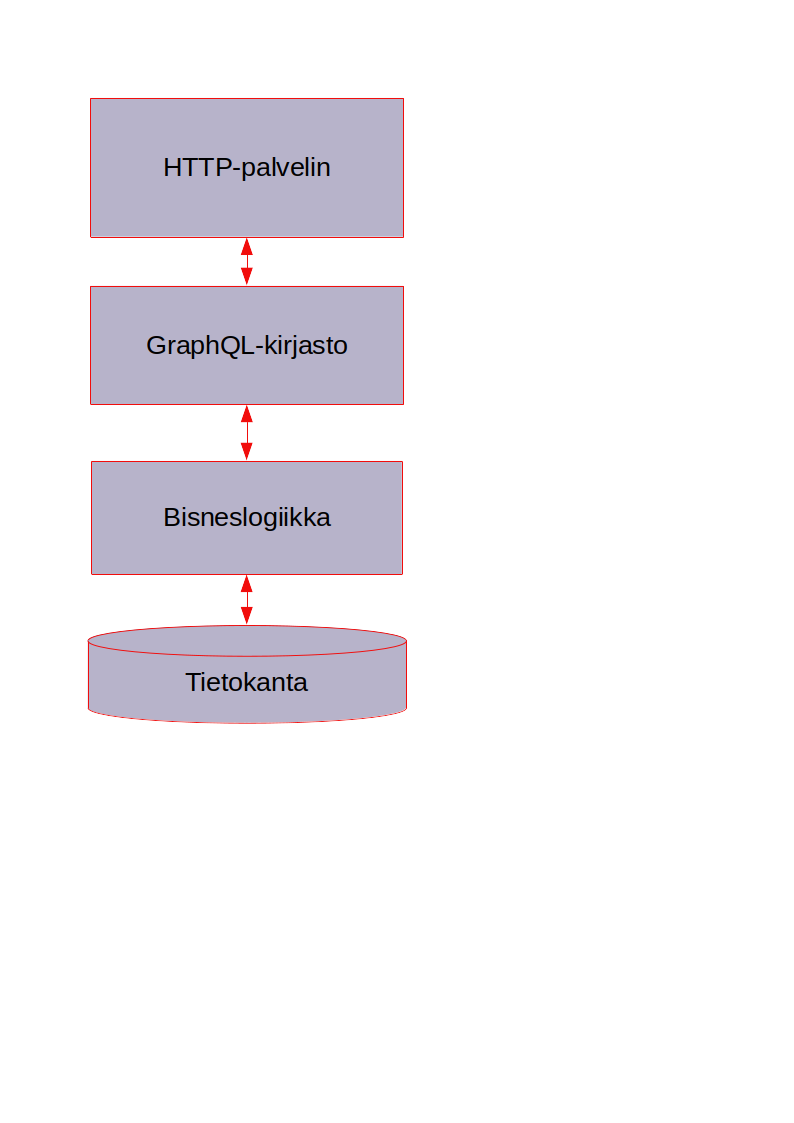
\includegraphics{illustration/GraphQL-arkkitehtuuri.png}
\caption{\label{graphqlarkkitehtuuri} Esimerkkiarkkitehtuuri
GraphQL-sovellukselle}
\end{figure}

Kuvassa \ref{graphqlarkkitehtuuri} esitän yksinkertaisen
GraphQL-sovelluksen arkkitehtuurin. Arkkitehtuuri on kerroksittainen, ja
rajapinnalle esitettävä pyyntö liikkuu siinä ylhäältä alaspäin. Koska
GraphQL on teknologianeutraali, tämä on vain yksi, toki suhteellisen
tyypillinen esimerkki mahdollisesta GraphQL-sovelluksesta.

Ensiksi pyyntö saapuu HTTP-palvelimeen. Tämä palvelin on käytännössä
ohjelmointikielestä riippuen kirjasto, joka vastaanottaa HTTP-pyyntöjä
ja osaa käsitellä niitä. Tyypillisesti GraphQL-rajapinnassa on vain yksi
\texttt{graphql}-niminen resurssi, jolle pyynnöt esitetään. Pyynnöt ovat
aina POST-tyyppisiä.

HTTP-kerros ottaa pyynnön vastaan ja lukee sen body-osassa olevan
merkkijonomuotoisen GraphQL-kyselyn. Tämä kysely on tehty
GraphQL-kyselykielellä. Rajapinta antaa kyselyn GraphQL-kirjastolle.

Kirjasto ottaa kyselyn vastaan ja tarkistaa sen oikeellisuuden
GraphQL-skeemaa vasten. Mikäli kysely on muodoltaan oikeanlainen,
kirjasto ohjaa sen eteenpäin resolvereiksi kutsutuille funktioille.
Resolver-funktiot eivät ole osa kirjastoa, vaan sovelluksen kehittäjä
kirjoittaa ne. Käytännössä resolver-funktio on nk. \gls{puhdasfunktio},
jonka tehtävänä on tuottaa vastaus yksittäiseen GraphQL-kyselyn
kenttään.

Laskutusta käsittelevässä esimerkissä rajapinnan invoices-kenttää voisi
vastata \texttt{invoices\_resolver}-niminen funktio.

Resolver-funktioiden kerros on alin kerros, josta GraphQL-palvelu
tietää. Sen alla oleva ohjelmistologiikka on riippumaton rajapinnan
olemassaolosta. Tyypillisesti siellä voi sijaita sovelluksen
liiketoimintalogiikka ja infrastruktuuri, kuten esimerkiksi tiedon
tallennusteknologia.

\hypertarget{query-ja-mutation--juurityypit}{%
\subsection{Query ja Mutation
-juurityypit}\label{query-ja-mutation--juurityypit}}

GraphQL-palveluissa on muutama oletuksena määritelty tyyppi, joita
kutsutaan juurityypeiksi. Tässä käsittelen niistä kahta keskeisintä,
Query- ja Mutation-tyyppiä.

Rajapintaan voi tehdä kyselyjä Query-tyyppisen juuriolion kautta. Tämän
olion kentät määrittävät, mitä dataa rajapinnalta voidaan kysellä.
Kentät ovat ikäänkuin sisäänmenoaukkoja, joiden kautta oliorakenteita
voi pyytää.

Kun aiemman koodiesimerkin \ref{listing1} mukaisesti määritellystä
GraphQL-rajapinnasta halutaan hakea tietoja, tehdään Query-tyypin
consolidatedInvoices-kenttään kysely, joka kuvaa halutun oliopuun
rakenteen tyyppien avulla. Tätä kuvaa koodiesimerkki \ref{listing2}.

\begin{code}
  \begin{minted}{graphql}

{
  consolidatedInvoices {
    number
    invoices {
      number
      sum
    }
  }
}
\end{minted}
\captionof{listing}{Kysely, joka pyytää consolidatedInvoices-olioita}
  \label{listing2}
\end{code}

Kyselyssä määritellään kentät, jotka palautuvassa datassa halutaan
nähdä. Näin myös palautuvan oliopuun syvyyttä voidaan kontrolloida.
Oheisessa esimerkissä haetaan paitsi lista koontilaskuista, myös
jokaisen koontilaskun alle invoices-kenttään lista siihen kuuluvista
laskuista. Niistä pyydetään jokaisesta laskunumero ja laskun summa. Näin
edetään verkkoa pitkin tarvittavan datan luo.

Mutation-juurityyppiä puolestaan käytetään datan muunnoksiin.
Mutation-tyypin sisältämiin kenttiin lähetetään kysely, jossa mukana
olevat parametrit kertovat, miten dataa muokataan. Parametrit ovat yhtä
lailla tyypitettyjä kuin rajapinnan kentät, ja GraphLQ-kirjasto
tarkistaa niiden tyypin oikeellisuuden. Mutation-komennot voivat myös
palauttaa oliorakenteita.

Oheisessa koodiesimerkissä \ref{listing3} määritellään invoice-niminen
operaatio uuden laskun luomiseen. Operaatiolle on merkitty paluuarvo,
joka on Invoice-tyyppinen olio. Käytännössä operaatio siis palauttaa
juuri luodun laskun.

\begin{code}
  \begin{minted}{graphql}
Mutation {
  invoice(customerId: Int, appointmentDate: String): Invoice
}
\end{minted}
\captionof{listing}{Esimerkki GraphQL-mutaatiosta}
  \label{listing3}
\end{code}

Kun tällaista mutaatiota käytetään, kutsuun liitetään myös kyselyosa,
jossa listataan ne kentät, jotka palautuvasta oliosta halutaan.
Koodiesimerkissä \ref{listing4} pyydetään laskunumero ja laskun summa.

\begin{code}
  \begin{minted}{graphql}

{
invoice(customerId: 1, appoitnmentDate: "2021-09-21") {
    number
    sum
  }
}
\end{minted}
\captionof{listing}{Esimerkki parametreja käyttävästä GraphQL-kyselystä}
  \label{listing4}
\end{code}

\hypertarget{graphql-ja}{%
\section{\texorpdfstring{GraphQL ja
\glsentrytext{ddd}}{GraphQL ja }}\label{graphql-ja}}

Eric Evansin kirjassa \glsentrytext{domainmodel} rakennetaan
olio-ohjelmoinnin tekniikoita käyttäen. Vaikka se ei olekaan ainoa tapa
rakentaa \glsentrytext{domainmodel}, on se kuitenkin tyylinä hyvin
suosittu.

Kuten edellä olen esittänyt, GraphQL puolestaan on olioverkkoon
perustuva rajapinta, jossa rajapinnan tarjoama tieto on jäsennetty
olioiksi ja niiden välisiksi suhteiksi.

Voidaan siis esittää kysymys, kuinka hyvin GraphQL-rajapinta soveltuu
\glsdisp{ddd}{sovellusaluevetoisen suunnittelun} tarpeisiin. On helppo
kuvitella, että olioverkolla on mahdollista heijastaa
\glsentrytext{domainmodel}, ja jopa mallintaa se lähes yksi yhteen.
Toisaalta GraphQL-rajapinta palauttaa dataa, kun taas olio-ohjelmoinnin
keinon luotu olioverkko voi esittää dynaamisen ja muuttuvan mallin. Onko
GraphQL toimiva väline ohjelmiston tietomallin parantamiseen? Tätä
kysymystä lähden työni käytännön osassa selvittämään.

\hypertarget{tyuxf6n-kulku}{%
\chapter{Työn kulku}\label{tyuxf6n-kulku}}

Yrityksessä haluttiin valita laskutuksen sisältä tapaus, jossa
hoitokäynti tulee voida jakaa usealle eri maksajalle osoitetuille
laskuille, ja nämä laskut tulee voida hyvittää itsenäisesti.

Mallintamisen aiheeksi valittu laskutus oli aihealueena minulle
tuntematon, ja yksi prosessin haasteita olikin, pystynkö muutamassa
viikossa omaksumaan riittävästi laskutuksen käsitteitä toimivan mallin
aikaansaamiseksi.

\hypertarget{laskutuksen-taustaa}{%
\section{Laskutuksen taustaa}\label{laskutuksen-taustaa}}

Ohjelmistoa käyttävä terapeutti kirjaa järjestelmään hoitokäyntejä ja
laskuttaa niitä. Monesti samalle maksajalle - etenkin, jos tämä ei ole
yksityishenkilö vaan instituutio - kertyy monta eri laskua, jotka
lähetetään yhtenä joukkona esimerkiksi kerran kuukaudessa. Tätä
kutsutaan koontilaskuksi.

Toisinaan jo luodussa laskussa huomataan virhe. Kirjanpidon
periaatteiden mukaan laskuja ei kuitenkaan saa tuhota, vaan virheellinen
lasku on oikaistava tai kumottava. Tässä ohjelmistoprototyypissä
oletetaan, että kyse on aina virheellisesti laskutetusta käynnistä, jota
maksaja kieltäytyy maksamasta, ja joka pitää kumota. Tämä tapahtuu
luomalla hyvityslasku.

Hyvityslasku on voitava luoda siten, että yksittäisellä laskulla oleva
yksittäinen rivi voidaan kumota, muun laskun (ja sen sisältävän
koontilaskun) säilyessä avoimena.

\hypertarget{tyuxf6skentelytavat}{%
\section{Työskentelytavat}\label{tyuxf6skentelytavat}}

Päätin tehdä työn lyhyissä iteraatioissa, ketterän kehityksen
periaatteita seuraten. Tämä tyyli soveltuu hyvin yhteen tietomallin
kehittämisen kanssa, sillä Evansin kirjassa kuvattu työtapa on
samankaltainen. Lisäksi lyhyet iteraatiot ovat nykyään tyypillinen tapa
tehdä ohjelmistoa.\cite{ConsultancyEu2020May}\cite{AgileIteration} En
asettanut iteraatioille mitään ennalta määrättyä kestoa.

Sovellusaluevetoisessa suunnittelussa oleellista on ohjelmoijan ja
sovellusalueen asiantuntijan välinen kommunikaatio. Asetin siis tiimimme
tuoteomistaja Lauran sovellusalueen asiantuntijan rooliin, ja käytin
häntä kuvitteellisen asiakkaan edustajana. Tämä rooli sopi Lauralle
erinomaisesti johtuen hänen työkokemuksestaan fysioterapeuttina ja
yritäjänä.

Malli laadittiin englanninkielisillä käsitteillä, koska Nordhealth on
viime vuosina laajentanut toimintaansa ulkomaille, ja yrityksen
viralliseksi kieleksi on vaihdettu englanti.

Päätin, että jokainen iteraatio aloitetaan minun ja tuoteomistaja Lauran
välisellä suunnittelukokouksella, jonka pääasiallisena tavoitteena oli
keskustellen ja piirtäen etsiä toimivaa ohjelmiston tietomallia.
Prosessin kuluessa tavaksi vakiintui, että kokouksen aluksi käytiin
nopeasti läpi siihen asti aikaansaadun ohjelmistoprototyypin
toiminnallisuus.

Pyrin noudattamaan työskentelyssä Eric Evansin esittämää tiedon
rouhimisen periaatetta, jossa suunnittelu ja ohjelmistokehitys
limittyvät keskenään. Iteraation aikana ohjelmoin uuden version
ohjelmistoprototyypistä, kokouksessa syntyneiden ajatusten pohjalta.
Kehitin ohjelmistoa testivetoisesti: kirjoitin ensin epäonnistuvan
yksikkötestin ja sen jälkeen tuotantokoodia sen verran, että
yksikkötestin suorittaminen onnistui. Käytin valmistunutta prototyyppiä
jatkokeskustelujen pohjana.

\hypertarget{teknologiavalinnat}{%
\section{Teknologiavalinnat}\label{teknologiavalinnat}}

Kirjoitin esimerkkiohjelmiston tyypilliseksi web-sovellukseksi, jossa
palvelinohjelmisto ja selaimessa toimiva asiakasohjelma kommunikoivat
keskenään HTTP-pyyntöjen avulla. Valitsin palvelinohjelmiston
kehityskieleksi Python-kielen, koska sitä käytetään Nordhealthilla
muutenkin. Python on myös syntaksiltaan suoraviivainen ja tässä mielessä
helppokäyttöinen, prototyyppien rakentamiseen soveltuva kieli.

Pythonin kanssa käytettäväksi HTTP-kirjastoksi valitsin
Falcon-kirjaston\cite{FalconPython} puhtaasti sen yksinkertaisuuden
vuoksi. Muita vaihtoehtoja olivat Django ja Flask\cite{FlaskPython},
mutta molemmat niistä sisälsivät paljon toimintoja, joita ei tässä
projektissa tarvittu. Niissä on mukana esimerkiksi tuki sivupohjille,
jota rajapintaa kehitettäessä ei tarvita. Ohjelmaan tarvittiin tuki vain
yhdelle HTTP-resurssille, joka vastaa pyyntöihin JSON-muotoisella
dokumentilla. GraphQL-kirjastoista harkitsin
Ariadne\cite{AriadnePython}- ja Graphene\cite{GraphenePython}
-kirjastojen välillä. Valitsin Ariadnen, koska se on tarkoitettu skeema
edellä tapahtuvaan kehitystyöhön.

Yksikkötestijärjestelmänä käytin Pytest-kirjastoa. Tietokantaa
sovellukselle ei tarvittu, vaan rakenteet voidaan tallentaa muistiin
ajonaikaisesti. Tämä helpottaa myös ohjelmiston tietorakenteen
refaktorointeja, sillä tietokantaa ei ole tarve muokata tai luoda
uudelleen ohjelmiston mallin muuttuessa.

Asiakassovelluksen kirjoitin Vue.js -JavaScript-kirjastoa käyttäen,
koska se on Nordhealthilla käytössä jo ennestään. GraphQL-rajapinnan
kanssa kommunikoimiseen käytin Apollo-kirjastoa, ja sen Vueen
integroivaa Vue Apollo -kirjastoa.

\hypertarget{kuvaus-prosessin-etenemisestuxe4-iteraatio-iteraatiolta}{%
\section{Kuvaus prosessin etenemisestä iteraatio
iteraatiolta}\label{kuvaus-prosessin-etenemisestuxe4-iteraatio-iteraatiolta}}

Esitän seuraavaksi prosessin etenemisen iteraatio kerrallaan. Olen
valinnut tähän osuuteen päiväkirjamaisen ja epämuodollisen tyylin, jonka
kautta pyrin kuvaamaan prosessin luonnetta. Ohjelmiston kehittäminen
koostui vapaamuotoisista keskusteluista, joihin kuului paljon kokeiluja
ja hapuiluja eri suuntiin. Tämä tyyli oli oma pyrkimykseni synnyttää
tiedon rouhimisen prosessi.

Malleja esittävissä kuvissa käyttämäni notaatio on hyvin alkeellinen,
eikä millään tapaa muodollinen. Se muistuttaa etäisesti UML-kielen
luokkakaavioita, ja sen keskeisin tarkoitus on luoda jaettu ymmärrys eri
käsitteiden välisistä suhteista.

\hypertarget{iteraatio-1-projekti-kuxe4ynnistyy-kirjanpidon-alkeita}{%
\subsection{Iteraatio 1: projekti käynnistyy, kirjanpidon
alkeita}\label{iteraatio-1-projekti-kuxe4ynnistyy-kirjanpidon-alkeita}}

Iteraation aloittavassa kokouksessa kävimme läpi laskutuksen
perusperiaatteita. Käsittelimme laajasti koko ongelmakenttää, ja
pohdimme mahdollisia ratkaisuja laskutuksen liepeillä oleviin
kysymyksiin. Näistä monet jäivät toteutetun prototyypin ulkopuolelle,
mutta ne selkiyttivät käsitystä ongelmakentän luonteesta.

Laura selitti kärsivällisesti kirjanpidon alkeita, jotka olivat minulle
enimmäkseen uutta tietoa. Keskeinen oivallus oli, että kirjanpidossa
kirjanpitoaineistoa ei saa luomisen jälkeen enää muuttaa. Jos laskua
halutaan myöhemmin korjata, on luotava erillinen kirjanpitotosite, jolla
oikaisu tehdään. Tätä kutsutaan tässä yhteydessä hyvityslaskuksi.

\begin{figure}
\centering
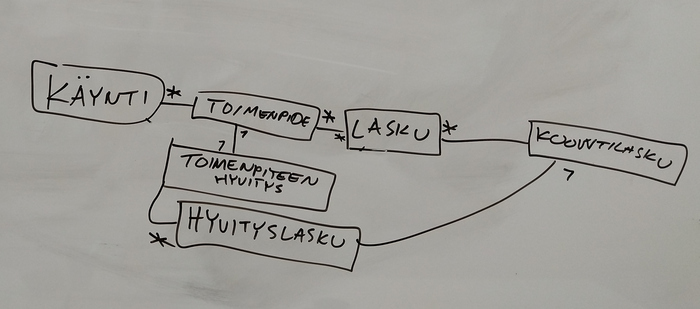
\includegraphics{illustration/malli1.jpg}
\caption{\label{malli1} Ensimmäinen malli}
\end{figure}

Suunnittelimme yksinkertaisen mallin, jossa hoitokäynnit liittyvät
laskuihin ja laskut kootaan koontilaskuille. Yksittäiset käynnit voidaan
lisätä myös hyvityslaskulle. Tämän mallin tarkoituksena oli luoda
yksinkertainen esimerkkisovellus, joka kykenee laskuttamaan käyntejä, ja
sen jälkeen lisäämään niitä hyvityslaskulle, sekä näyttämään
hyvityslaskun kokonaissumman. Malli on esitetty kuvassa \ref{malli1}.

Tämän mallin sisältävän ohjelmistoprototyypin toteuttamiseen kului kaksi
viikkoa, ja näin iteraatio oli prosessin pisin. Myöhemmät iteraatiot
kestivät noin viikon. Kulunutta aikaa selittää, että rakensin
prototyypin puhtaalta pöydältä, jolloin aikaa kului myös sovelluksen
pohjan pystyttämiseen.

Ensimmäisessä iteraatiossa syntynyt ohjelmisto ei malliltaan täysin
vastannut tätä ensimmäisen kokouksen piirrosta. Yksinkertaisuuden vuoksi
oletin, että käynnillä on aina vakiohintainen toimenpide, jolloin
Toimenpide-olio jäi mallista pois. Tehdessä huomasin myös, että
koontilaskun ja hyvityslaskun välille ei tarvita mitään suoranaista
yhteyttä. Riittää, että käynti on yhdistetty näihin molempiin.

\hypertarget{iteraatio-2-malli-syvenee}{%
\subsection{Iteraatio 2: malli
syvenee}\label{iteraatio-2-malli-syvenee}}

Iteraation aloittavassa kokouksessa kävimme läpi syntyneen
ohjelmistoprototyypin. Läpikäynnin jälkeen olin hieman epävarma, miten
tapaamista tulisi jatkaa. Päätin ottaa puheeksi minua koko viikon ajan
vaivanneen käyntien ja laskujen läheisen kytköksen. Ohjelmoidessa tuntui
väärältä ja kömpelöltä, että käynti lisätään suoraan laskulle ja vielä
hyvityslaskullekin.

Pyysin Lauraa kertomaan enemmän siitä, mitä käynnin laskuttaminen
oikeastaan tarkoittaa, ja hän kuvasi, millaisissa tilanteissa laskuja
voidaan luoda. Huomioni kiinnittyi puheessa esiintyneeseen termiin
\textbf{Laskutusperuste}. Tämä tuntui valtavan kiinnostavalta, ja Laura
avasi asiaa tarkemmin. Kun laskulle lisätään laskutettavia asioita,
täytyy siihen olla jokin peruste.

\begin{figure}
\centering
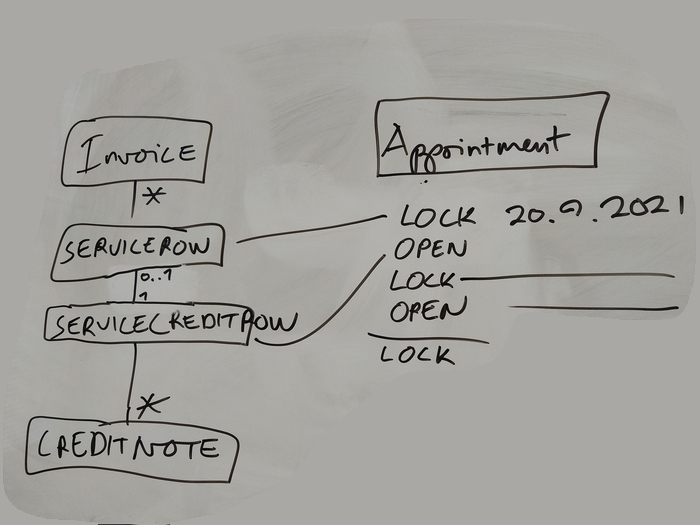
\includegraphics{illustration/malli2.jpg}
\caption{\label{malli2}Toinen malli}
\end{figure}

Käytimme tapaamisen loppuosan tämän idean kehittelemiseen. Päädyimme
ajatukseen, jossa laskulle lisätään käynnin sijasta palvelurivi, joka
viittaa käyntiin. Tapaamisen jälkeisen viikon kehitystyötä ohjasi nyt
uusi ajattelutapa: käyntiä sinänsä ei liitetä laskuun, vaan käynti
laskutetaan, mikäli laskutusperuste täyttyy.

Yksi toisen tapaamisen aikana syntyneistä malleista on esitetty kuvassa
\ref{malli2}. Siinä laskulle liitetään palvelurivi, joka vastaa
yksittäistä hoitokäyntiä. Mikäli käynti hyvitetään, palveluriviä vastaa
hyvityslaskuun kiinnitetty hyvitysrivi.

Kuvan laidassa näkyy myös hahmotelma siitä, miten käynnin voisi
hyvittämisen jälkeen laskuttaa uudelleen. Sarja monimutkaisia
lukitusoperaatioita tuntui Laurasta jo piirtämisen yhteydessä hankalalta
ymmärtää. On myös kuvaavaa, että pidimme tapaamisen aikana tätä
syntynyttä mallia puutteellisena, ja kehitimme siitä mielestämme
paremman version.

Mallin toteuttamisessa kesti vajaat neljä päivää. Jotta uusi ajatus
palvelurivistä oli mahdollista lisätä koodiin, täytyi olemassaolevaa
ohjelmaa aluksi refaktoroida voimakkaasti. Aiemmin suoraan laskulle
kytkettyyn käyntiin piti sijoittaa sisälle palveluriviä kuvaava olio, ja
lasku muuttaa koostumaan näistä. Käynnin ja hyvityslaskun välinen kytkös
piti katkaista, ja tilalle rakentaa kytkös laskurivin ja hyvitysrivin
välille.

Koodin refaktoroimisessa kului aluksi päivä, ja sen jälkeen uuden,
palvelurivejä ja hyvitysrivejä käsittelevän koodin luomiseen kaksi
päivää.

Perjantaihin tultaessa olin refaktoroinut prototyyppiohjelmaa ja sen
jälkeen käyttänyt kolme päivää ensimmäisen käyttäjätarinan parissa.
Vaikutti, että aikataulu pettää, eikä mitään tule valmiiksi maanantaille
sovittuun seuraavaan tapaamiseen.

\begin{figure}
\centering
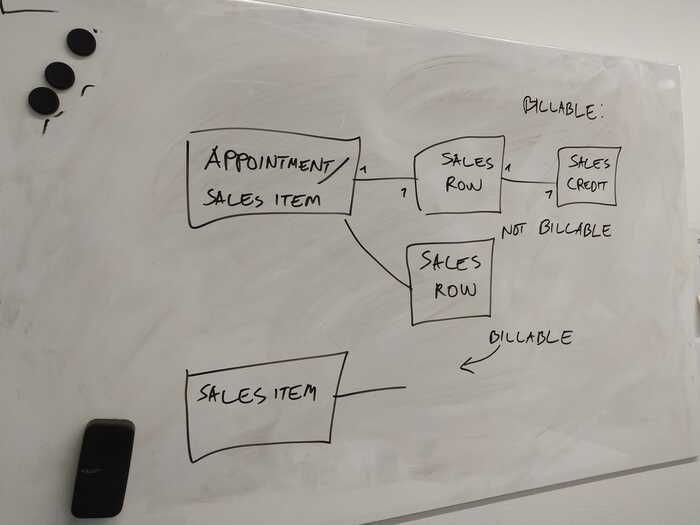
\includegraphics{illustration/final-idea-1.jpg}
\caption{\label{finalmodel1} Kuva, jossa käyntiin kytkeytyy palvelurivi
ja palveluriviin hyvitysrivi}
\end{figure}

Yllättäen perjantaina puolen päivän jälkeen kaikki yksikkötestit menivät
läpi, käyttäjätarina valmistui, ja ohjelmistoprototyypin toiminnassa
tuntui tapahtuvan laadullinen hyppäys. Vaikutti, kuin prototyyppiohjelma
olisi oppinut itsekseen jotain laskutuksesta. Ohjelman logiikka toimi
paremmin kuin mitä itse ymmärsin laskutuksesta.

Loppujen kahden käyttäjätarinan toteuttaminen onnistui kahdessa
tunnissa, ja vaati vain joitain rivejä koodia.
\Glsentryname{domainmodel} oli syventynyt.

Ohjelmoidessa syntynyt tietomalli sisälsi samat asiat, joista
kokouksessa oli puhuttu, mutta niiden suhteet olivat toisenlaiset. Olin
tuottanut ominaisuudet yksikkötesti yksikkötestiltä, ja tämä malli oli
yksinkertaisin, jolla kaikki testit menivät läpi. Malli on esitetty
kuvassa \ref{finalmodel1}

\hypertarget{iteraatio-3-malli-osoittaa-joustavuutensa}{%
\subsection{Iteraatio 3: malli osoittaa
joustavuutensa}\label{iteraatio-3-malli-osoittaa-joustavuutensa}}

Kolmannen iteraation aluksi pidimme jälleen suunnittelukokouksen. Tämän
tapaamisen keskeisimpänä ongelmana oli, miten jo kertaalleen laskutettu
ja hyvitetty käynti voidaan laskuttaa uudelleen.

Yritimme piirtää monenlaisia erilaisia malleja ja diagrammeja, mutta
mikään niistä ei tuntunut osuvalta. Tämä tapaaminen oli tunnelmaltaan
kaikista tapaamisista jähmein. Kun kommunikaatio ei sujunut, myöskin
malli kehittyi kehnosti.

Laadimme tapaamisen lopuksi kuitenkin joukon käyttäjätarinoita, jotka
tähtäsivät tavoitteeseemme, hyvitetyn käynnin uudelleenlaskuttamiseen.

Aloitin myös tämän viikon ohjelmointityön samantapaisella mallin
refaktoroinnilla kuin edellisen. Tällä kertaa se oli suppeampi, koska
uusia ajatuksia oli vähemmän.

Ohjelmoidessa yllätyin: sain rakennettua yhdessä päivässä ominaisuuden,
jossa kertaalleen laskutettu ja hyvitetty käynti voidaan laskuttaa
uudelleen. Käytännössä riitti, että muutin käynnillä olevan viittauksen
palveluriviin listamuotoiseksi. Nyt käyntiin oli mahdollista kytkeä
yhden sijasta monta eri palveluriviä, jolloin uudelleenlaskutus
onnistui. Palvelurivien, ja niihin kytkeytyvien hyvitysrivien suhteista
oli helppo rakentaa säännöt sille, onko käynti laskutettavissa vai ei.

Tämä listamuoto on esitetty kuvassa \ref{finalmodel1}. Siinä
tarkastellaan palvelurivien listan viimeisintä jäsentä, ja tällä
perusteella arvioidaan, onko käynti laskutettavissa vai ei.

Kolmas iteraatio oli iteraatioista lyhin, ja se kesti vain noin neljä
päivää.

\hypertarget{iteraatio-4-piilossa-ollut-kuxe4site-luxf6ytyy}{%
\subsection{Iteraatio 4: piilossa ollut käsite
löytyy}\label{iteraatio-4-piilossa-ollut-kuxe4site-luxf6ytyy}}

Neljännen tapaamisen keskeinen ongelma oli, että käynti tuntui olevan
edelleen liian vahvasti kytketty laskuun. Yksittäistä käyntiä vastasi
yksi palvelurivi. Tämä käy ongelmalliseksi, mikäli käynti halutaan jakaa
kahdelle maksajalle. Jo ensimmäisessä tapaamisessa oli käynyt selväksi,
että ainut siisti tapa jakaa käynti kahdelle maksajalle on tehdä kaksi
erillistä laskua. Käyntiin kytkettyä palveluriviä ei kuitenkaan voi
lisätä molemmille laskuille.

Vaikutti siltä, että käynnin ja laskun välistä puuttui edelleen jokin
käsite. Olin keskustellut aiemmin viikolla laskutuksen kanssa
työskennelleen tiimikaverini kanssa, ja hän kiinnitti huomiota siihen,
että laskuille laitettiin ``palvelurivejä''. Hän oli itse käyttänyt
omissa malleissaan ``myyntiä''.

Nyt muistin tämän keskustelun, ja ehdotin sen pohjalta, että
laskutuksessa ei käsiteltäisikään suoraan käyntejä vaan palvelumyyntiä.
Laura totesi, että kaikki laskuille laitettava on lopulta myyntiä ---
ikäänkuin se olisi ollut itsestäänselvyys! Ohjelmoijalle tämä oivallus
oli kuitenkin uusi tieto, ja se avasi täysin uuden näkökulman
laskutukseen.

\begin{figure}
\centering
\includegraphics{illustration/malli4.jpg}
\caption{\label{malli3}Kolmas malli}
\end{figure}

Loimme kokouksessa mallin, jossa käynti muunnetaan myynniksi eli
SalesItem-olioksi. Nyt käynneistä ei tarvitse välittää lainkaan laskuja
käsiteltäessä. SalesItem puolestaan voidaan jakaa maksajille
suunnatuiksi osuuksiksi, SalesShareiksi, ja yksittäisellä laskulla on
SalesShareen kytketty SalesRow. Malli on esitetty kuvassa \ref{malli3}

Kokouksen jälkeen minua odotti jälleen refaktorointityö, joka oli
projektin suurin. Käynnin perinpohjainen irrottaminen koko
laskutuslogiikasta ja kahden uuden käsitteen laittaminen näiden väliin
vaativat laajan remontin koko ohjelman toimintalogiikkaan.

Uusien ominaisuuksien toteuttaminen refaktoroinnin jälkeen oli
huomattavan suoraviivaista, ja tuloksena syntyi ohjelma, joka pääsi
alkuperäiseen tavoitteeseensa, jaetun käynnin hyvittämiseen ja uudelleen
laskuttamiseen. Ohjelma oli muutamassa viikossa laajentunut yllättävän
monipuoliseksi, vaikka sitä ei pinnalle päin heti huomannutkaan.

\hypertarget{huomioita-prosessista}{%
\section{Huomioita prosessista}\label{huomioita-prosessista}}

Pienen prototyyppiohjelman kehittäminen oli valtavan hyödyllistä, ja se
tuotti tukun tärkeitä oivalluksia siitä, miten sovellusaluevetoista
suunnittelua tehdään, ja mikä on GraphQL:n merkitys prosessissa.

Mallia kehittäessä vaadittujen voimakkaiden refaktorointijaksojen määrä
yllätti. Ennalta kirjallisuudesta luettuna ei refaktoroinnin määrää
ollut helppo hahmottaa. Omakohtainen tekeminen paljasti, miten
oleellinen osa \glslink{ddd}{Sovellusaluevetoista suunnittelua}
refaktorointien tekeminen on.

Refaktoroiminen ei ole tässä tyylissä pelkästään tekninen keino pitää
koodia siistinä, vaan strateginen väline, jonka avulla mallia
parannetaan ja \glslink{ubilang}{kaikenkattavaa kieltä} kehitetään.

Toinen keskeinen keino kaikenkattavan kielen kehittämiseen tässä
prosessissa oli suunnittelutapaamistemme kielen tarkka seuraaminen.
Pyrin nappaamaan Lauran kanssa käydyistä keskusteluista termejä, joita
käytimme, ja etenkin termejä, joita Laura käytti.

Eric Evans mainitsee, että \glsdisp{ubilang}{kaikenkattavan kielen}
rakentamisessa oleellista on löytää sanat, joita alan asiantuntijat
käyttävät. Etenkin puuttuvien käsitteiden tunnistaminen puheen seasta
auttaa paljon mallin parantamisessa.\cite{evans:ddd}

\hypertarget{kuxe4sitteiden-hyuxf6dyntuxe4minen}{%
\section{\texorpdfstring{\glsdisp{ddd}{Sovellusaluevetoisen suunnittelun}
käsitteiden
hyödyntäminen}{ käsitteiden hyödyntäminen}}\label{kuxe4sitteiden-hyuxf6dyntuxe4minen}}

Käytin tietomallin koodia rakentaessani apuna Evansin esittelemiä
käsitteitä. Useat käsitteet, kuten käynnit ja laskut, kuvasin
\glslink{entity}{yksilötyyppeinä}. Käsitteistä koostuvat kokonaisuudet
ovat \glsdisp{aggregate}{aggregaatti}-rakenteissa. Esimerkiksi laskun
sisältämät laskurivit tai myynnin sisältämät myyntiosuudet.

Koska yksinkertaisessa prototyyppisovelluksessani ei ole ollenkaan
tietokantaa, toteutin käsitteille Evansin mallin mukaisesti
\glsdisp{repository}{repositoriot}. Käytännössä ne ovat vain
yksinkertaisia luokkia, jotka pitävät sisällään linkitetyn listan
olioita.

Laskujen luominen puolestaan oli operaationa niin monimutkainen, että
siihen tarvitsin Eric Evansin esimerkin mukaisesti erillisen
tehdasluokan. Senkin jälkeen operaatio oli melko monimutkainen. Vielä
prototyyppiohjelman kehityksen päättyessä minulla oli vahva tunne, että
tehdasluokkaan jääneet sotkuiset koodin osat olivat seurausta jostakin
puuttuvasta käsitteestä.

\hypertarget{graphql-rajapinnan-ja-sovellusaluemallin-yhteys}{%
\section{GraphQL-rajapinnan ja sovellusaluemallin
yhteys}\label{graphql-rajapinnan-ja-sovellusaluemallin-yhteys}}

GraphQL-skeemat tuntuivat heijastavan todella osuvasti rakentamiamme
käsitekarttoja. Useimmiten oli mahdollista siirtää rakentamamme
käsitteiden verkko sellaisenaan GraphQL-skeeman sisälle. Tein tämän
monesti ensimmäisenä osana ohjelmointijaksoa. Tämä myös tarkoitti, että
palvelinohjelman ja asiakasohjelman välinen rajapinta sai ensimmäisenä
kyvyt uuden käsitekartan version käsittelemiseen.

Koska GraphQL on riippumaton käytetystä ohjelmointikielestä, myös malli
irtautui niistä välittömistä teknologioista, joilla
prototyyppisovelluksen rakensin. Voidaan siis sanoa, että
GraphQL-rajapintakehityksessä sovellusalueen käsitteet saavat
merkittävämmän roolin kuin alla käytettävät täsmälliset
teknologiavalinnat.

Huonommin GraphQL-rajapinta kuvasi mallin dynaamisia muutoksia.
Mutaatioiden avulla voidaan ilmaista, minkälaisia toimintoja malliin
voidaan kohdistaa, ja toiminnon onnistuminen voidaan toki havaita
muuttuneena mallina. Rajapinnasta ei kuitenkaan suoraan päällepäin näe,
missä ovat mallin dynaamiset nivelkohdat.

Esimerkiksi laskutusta käsittelevässä mallissa tällainen nivelkohta on
käynnin ja myynnin välissä. Kun käynti muuttuu myynniksi laskulle
lisättäessä, tapahtuu käsitteellinen muutos, joka antaa
prototyyppisovellukselle sen sisältämän voiman ja joustavuuden.

GraphQL-rajapinta myös lisäsi yhden ylimääräisen tason monimutkaisuutta:
skeemaa piti päivittää erikseen, mutta pelkillä skeeman muutoksilla ei
vielä ollut mahdollista selvittää mallin toimivuutta. Pelkästään
ohjelmakoodissa toteutettu sovellusaluemalli olisi ollut
yksinkertaisempi muokata. Toisaalta myös REST-rajapinta olisi
todennäköisesti tuonut vastaavaa monimutkaisuutta, kun sovellusaluemalli
olisi pitänyt esittää joukkona resurseja.

\hypertarget{tulokset}{%
\chapter{Tulokset}\label{tulokset}}

\hypertarget{prototyyppiohjelman-esittely}{%
\section{Prototyyppiohjelman
esittely}\label{prototyyppiohjelman-esittely}}

Prototyyppiohjelma on yksinkertainen yhden sivun selainsovellus. Sen
avulla voi luoda käyntejä, laskuttaa niitä, koota laskuja
koontilaskuiksi ja hyvittää yksittäisiä laskurivejä.

\begin{figure}
\centering
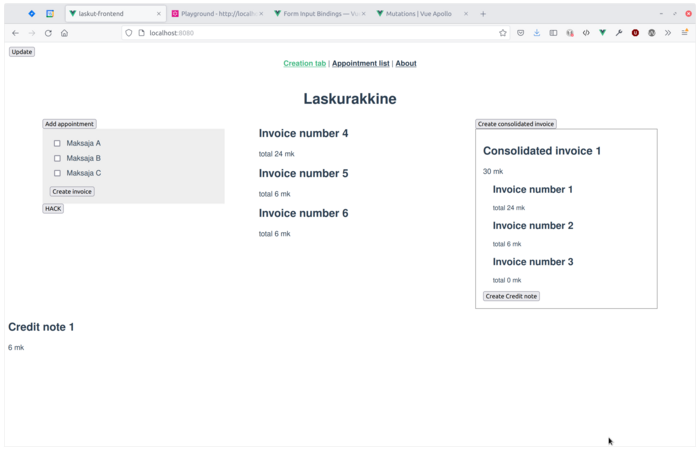
\includegraphics{illustration/screenshots/Laskurakkine.png}
\caption{\label{rakkine_default-view}Laskujen lisäysnäkymä}
\end{figure}

Ohjelman pääkäyttöliittymä on esitetty kuvassa
\ref{rakkine_default-view}

Laskujen sisältöjä voi tarkastella, ja ohjelma laskee laskujen avoimet
summat.

\begin{figure}
\centering
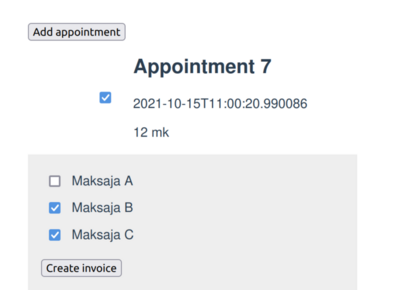
\includegraphics{illustration/screenshots/Dividing.png}
\caption{\label{rakkine_dividing}Esimerkki käynnin jakamisesta usealle
maksajalle}
\end{figure}

Lisäksi käyttöliittymästä voi valita maksajan luotavalle laskulle.
Mikäli maksajia valitaan useampia, ohjelma jakaa käynnit kahdelle eri
maksajalle. Tämä on esitetty kuvassa \ref{rakkine_dividing}.

\begin{figure}
\centering
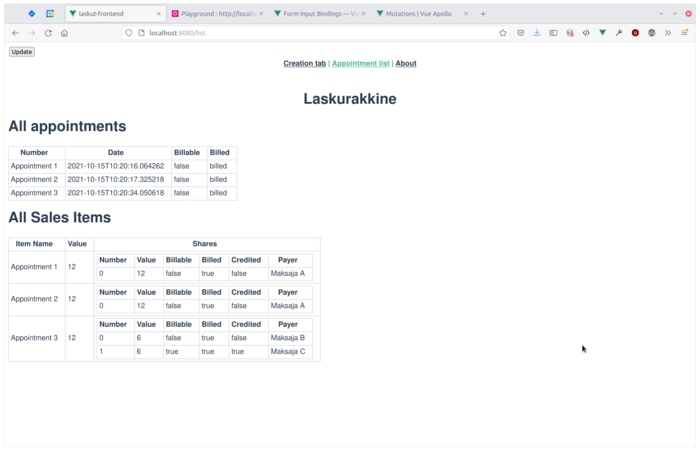
\includegraphics{illustration/screenshots/List-view.png}
\caption{\label{rakkine_list-view}Ohjelman listanäkymä}
\end{figure}

Erillisessä listanäkymässä (kuva \ref{rakkine_list-view}) voi
tarkastella luotujen käyntien tilaa sekä laskutettavan myynnin tilaa.
Ohjelma näyttää, onko käynti laskutettu vai laskuttamaton. Myynnin
osalta ohjelma näyttää, miten myynti jakautuu eri maksajille, ja onko
summa avoin, laskutettu vai hyvitetty.

\begin{figure}
\centering
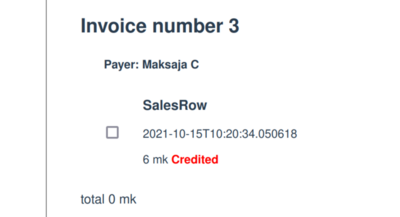
\includegraphics{illustration/screenshots/credited.png}
\caption{\label{rakkine_credited}Ohjelma näyttää, että yksittäinen
laskurivi on hyvitetty}
\end{figure}

Kuvassa \ref{rakkine_credited} on esitetty miten ohjelma näyttää
hyvitetyn laskurivin.

Käytin asiakasohjelman tekemiseen niin vähän aikaa kuin mahdollista. Se
näkyy tyylin hiomattomuutena. Luonnosmaisen näköinen ulkoasu myös
kommunikoi muille prosessiin osallistuville, että ohjelmisto tai
etenkään sen käyttöliittymä ei ole tarkoitettu tuotantokäyttöön, vaan
apuvälineeksi erilaisten tietomallin piirteiden kartoittamiseen.

\hypertarget{parannuksia-tietomalliin}{%
\section{Parannuksia tietomalliin}\label{parannuksia-tietomalliin}}

Viiden viikon aikana syntyi pieni malli laskutukseen tietorakenteen
parantamiseksi. Lisäksi löytyi kaksi pientä ideaa, joita voi hyödyntää,
kun ohjelmistoa kehitetään.

\begin{figure}
\centering
\includegraphics{illustration/malli4.jpg}
\caption{\label{finalmodel1-again}Lopullinen malli}
\end{figure}

Pieni malli laskutuksen parantamiseksi on esitetty kuvassa
\ref{finalmodel1-again}. Se pitää sisällään ajatuksen käynnin
muuttumisesta myynniksi, kun se saapuu laskutuksen piiriin. Oma
erikoisuutensa on myös käynnin jakamiseen liittyvä jakoperuste.

Prototyypissä emme ottaneet kantaa, millä perusteella käynnin hinnan
osittaminen eri maksajille tapahtuu. Käytännössä ohjelmassa on eri
maksajatahojen kanssa tehtyjä sopimuksia, jotka määrittelevät ehtoja
maksuosuuden suuruudesta. Jakoperuste on siis dynaamisesti muuttuva
käsite, joka riippuu haluttuihin maksajiin ja käyntiin kytkettyyn
hoitojaksoon yhdistyvistä sopimuksista.

\begin{figure}
\centering
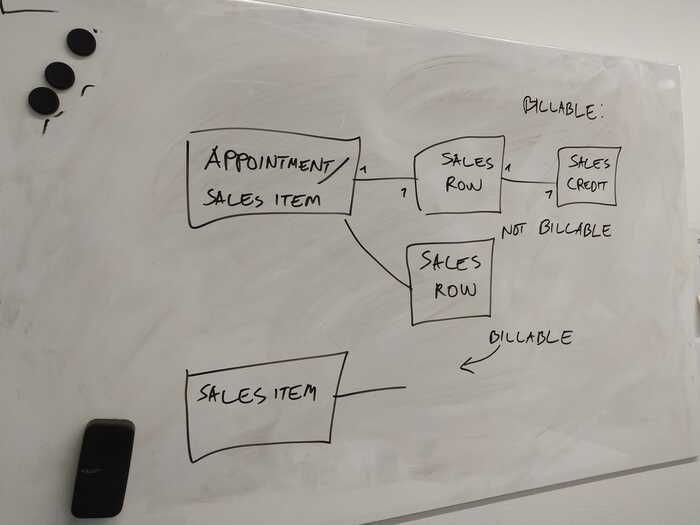
\includegraphics{illustration/final-idea-1.jpg}
\caption{\label{finalidea1}Idea 1}
\end{figure}

Kaksi pientä ideaa ovat molemmat käyttökelpoisia erillään mallista.
Ensimmäinen niistä on myynnin, myyntirivin ja hyvitysrivin välinen
tiivis yhteysketju. Tämä idea (kuva \ref{finalidea1}) mahdollistaa hyvin
yksinkertaisen ja joustavan myynnin laskutus- ja hyvityslogiikan.

\begin{figure}
\centering
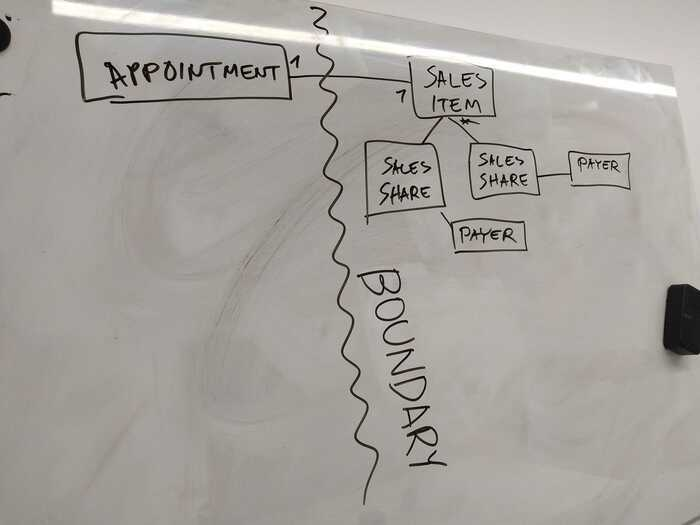
\includegraphics{illustration/final-idea-2.jpg}
\caption{\label{finalidea2}Idea 2}
\end{figure}

Toinen pieni idea on, että käynti kannattaisi erottaa selkeästi laskulle
tulevasta myynnistä. Tällöin on mahdollista myös esimerkiksi vaihtaa
myöhemmin maksajaa, jolta käynti laskutetaan ilman, että jo
muodostettuihin laskuihin tarvitsee kajota. Tämä ajatus on esitetty
kuvassa \ref{finalidea2}.

\pagebreak

\hypertarget{kuvaus-tyuxf6mallista}{%
\chapter{Kuvaus työmallista}\label{kuvaus-tyuxf6mallista}}

Tämän työn kuluessa syntyi työmalli, jota kutsun \emph{notkeaksi
tietomallin paranteluksi}. Työmalli on parhaimmillaan tilanteissa,
joissa ohjelmiston sovellusaluemalli sisältää monimutkaisia ja vain
erityisalan asiantuntijalle aukeavia käsitteitä ja käsitesuhteita.
Eduksi on myös, mikäli sovelluksen tekninen vaativuus ei ole kovin
poikkeuksellinen. Tyypillinen bisnessovellus, jossa painopiste on
sovellusalueessa, on hyvä kohde tälle työmallille.

Kuvaan seuraavassa tämän työmallin keskeiset ominaispiirteet.

\hypertarget{lyhyet-iteraatiot}{%
\subsubsection{Lyhyet iteraatiot}\label{lyhyet-iteraatiot}}

Lyhyet iteraatiot, joiden välissä pidetään suunnittelutapaaminen, ovat
ehdoton edellytys tietomallin ripeälle kehittämiselle. On tärkeää, että
iteraation kuluessa syntyy käyttökelpoinen ohjelmistoversio, jonka
avulla mallin toimivuutta voidaan testata ja todentaa.

\hypertarget{keskusteleva-suhde-tuoteomistajan-ja-kehittuxe4juxe4n-vuxe4lilluxe4}{%
\subsubsection{Keskusteleva suhde tuoteomistajan ja kehittäjän
välillä}\label{keskusteleva-suhde-tuoteomistajan-ja-kehittuxe4juxe4n-vuxe4lilluxe4}}

Koska tavoitteena on luoda kieli, jota voivat käyttää niin ohjelmoijat
kuin liiketoimintaväkikin, sen kehittämiseen luontevin ja
todennäköisesti ainoa tapa on rakentaa mallia keskustelevalla otteella.

\hypertarget{kuxe4yttuxe4juxe4tarinoihin-pohjautuva-tyuxf6lista}{%
\subsubsection{Käyttäjätarinoihin pohjautuva
työlista}\label{kuxe4yttuxe4juxe4tarinoihin-pohjautuva-tyuxf6lista}}

Ketterän kehityksen työkalupakista peräisin oleva ajatus
yksinkertaisista käyttäjätarinoista soveltuu hyvin tietomallin
kehittämisen lähtökohdaksi. Kun huomion keskipisteenä ovat ne asiat,
joita käyttäjä voi ohjelmistolla tehdä, on myös syntyvä malli lähempänä
alan realismia.

\hypertarget{keskittyminen-rajapinnan-rakenteeseen-ohjelmiston-rakenteen-sijasta}{%
\subsubsection{Keskittyminen rajapinnan rakenteeseen ohjelmiston
rakenteen
sijasta}\label{keskittyminen-rajapinnan-rakenteeseen-ohjelmiston-rakenteen-sijasta}}

Keskeinen kysymys työtä tehtäessä on, ilmaiseeko rajapinta
sovellusalueen ja ongelmakentän riittävän monipuolisesti. Teknisiin
yksityiskohtiin, ohjelmointikieliin ja kirjastoihin keskittymisen
sijasta huomio kannattaa pitää juuri rajapinnan ilmaisemassa
käsiteverkossa.

\hypertarget{rajapintaskeeman-rakentaminen-kuxe4sitteiden-pohjalta}{%
\subsubsection{Rajapintaskeeman rakentaminen käsitteiden
pohjalta}\label{rajapintaskeeman-rakentaminen-kuxe4sitteiden-pohjalta}}

GraphQL-rajapintaskeema kannattaa rakentaa ennenkuin kirjoittaa skeeman
toteuttavaa koodia. Näin kielen käsitteet ja niiden väliset suhteet
tulevat formaalisti ilmaistuksi. Ohjelmakoodin kirjoittamisen aikana
skeema saattaa myös tarkentua, ja silloin kannattaa muutokset tehdä
välittömästi.

\hypertarget{koodin-ja-mallin-pituxe4minen-luxe4hekkuxe4in}{%
\subsubsection{Koodin ja mallin pitäminen
lähekkäin}\label{koodin-ja-mallin-pituxe4minen-luxe4hekkuxe4in}}

Välttämätön osa tätä työtyyliä on koodin ja mallin vastaavuus. Mallissa
käytettävät käsitteet on löydyttävä koodista, ja koodissa tulisi olla
lähinnä vain nämä käsitteet ja niiden väliset suhteet sellaisina, kuin
ne \glslink{ubilang}{kaikenkattavassa kielessä} ilmenevät.

\hypertarget{voimakkaat-refaktoroinnit}{%
\subsubsection{Voimakkaat
refaktoroinnit}\label{voimakkaat-refaktoroinnit}}

Voimakkaat refaktoroinnit ovat keino muokata koodin esittämästä mallista
joustava ja ilmaisuvoimainen. Nämä refaktoroinnit vaativat ehdottomasti
tuekseen jämerän yksikkötestisetin. Sen rakentaminen onnistuu
käytännössä vain testit edellä tekemällä.

\hypertarget{ohjelmoinnissa-vastaan-tulleet-ongelmat-jatkosuunnittelun-luxe4htuxf6kohtina}{%
\subsubsection{Ohjelmoinnissa vastaan tulleet ongelmat jatkosuunnittelun
lähtökohtina}\label{ohjelmoinnissa-vastaan-tulleet-ongelmat-jatkosuunnittelun-luxe4htuxf6kohtina}}

Suunnittelutapaamisten ja ohjelmointiprosessin välinen yhteys ei saa
olla vain yksisuuntainen. Mikäli suunnittelutapaaminen nähdään ainoana
osana prosessia, jossa suunnittelua tapahtuu ja ohjelmointi pelkästään
suunnitelmien mekaanisena toteuttamisena, hyödyt tästä
työskentelytyylistä jäävät hyvin vähäisiksi. Ohjelmointiprosessi on
suunnittelutyön toisenlainen vaihe, ja siinä ilmenevät ongelmat ovat
oivallinen maaperä seuraavan suunnittelutapaamisen aiheiksi.

\hypertarget{tyuxf6mallin-haasteita}{%
\section{Työmallin haasteita}\label{tyuxf6mallin-haasteita}}

Tämä työmalli vaatii ohjelmoijalta paljon. Se edellyttää jatkuvaa
kiinnostusta sovellusalueen piirteistä, ja laajaa tarkkaavuutta
suunnittelutapaamisten keskuisteluissa. Lisäksi se edellyttää kykyä
sietää epävarmuutta ja muuttaa suunnitelmia usein ja isosti. Teknisellä
tasolla työmalli edellyttää kykyä joustavan ohjelmiston
suunnittelemiseen, laajojen refaktorointien tekemiseen kireässä
aikataulussa pysyen ja tiukkaa keskittymistä niihin päämääriin, jotka
mallin kehittämisessä on kulloinkin asetettu.

Jotta tällainen työmalli voi olla hedelmällinen tuotantotasoisen
ohjelmiston tekemisessä, se edellyttää myös, että työtyyli ohjelmoijan
ympärillä vastaa tällaista tekemisen tapaa. Liiketoimintavetoisella
suunnittelulla on vaikutuksia paitsi ohjelmistotuotannon prosessiin,
myös sitä ympäröiviin prosesseihin, kuten asiakastarpeiden kokoamiseen
ja tulevan kehitystyön suunnittelemiseen.

\hypertarget{yhteenveto}{%
\chapter{Yhteenveto}\label{yhteenveto}}

Tässä insinöörityössä pyrittiin kohentamaan ohjelmiston tietomallia
kehittämällä GraphQL-rajapinta
\glsdisp{ddd}{sovellusaluevetoisen suunnittelun} keinoin. Tavoitteena
oli parantaa nykyistä tietomallia ja luoda työprosessi tietomallin
parantelemiseen. Samalla etsittiin vastausta kysymykseen, miten hyvin
GraphQL-rajapinta teknologiana sopii tällaiseen prosessiin.

Saadakseni vastauksia kysymyksiin laadin pienen prototyyppisovelluksen,
jonka tehtäväksi asetimme yhdessä tilaajan edustajien kanssa
laskutukseen liittyvän konkreettisen ongelman ratkaisemisen. Keskeiset
vastaukset työn nostamiin kysymyksiin tulivat juuri tämän sovelluksen
kehitysprosessin kautta. Samalla kehitystyö muovasi lopullista
työprosessia.

Tehdyn kokeilun perusteella GraphQL-rajapinta soveltuu hyvin
sovellusaluevetoisen suunnittelun tarpeisiin. Tämä johtuu sen
verkkomaisesta luonteesta, jolla on helppo mallintaa sovellusalueen
käsitteiden keskinäisiä suhteita. Se, että GraphQL-verkko on nimenomaan
rajapinta, helpottaa käsitteellisen mallin erottamista omaksi
kokonaisuudekseen sovelluksen sisällä, ja irrottaa mallin
konkreettisesta teknologiasta.

Koska GraphQL-rajapinta määritellään \glsdisp{dsl}{täsmäkielen} avulla,
mallia on helppo muokata osana iteratiivista kehitysprosessia. Tämä
mahdollistaa tutkimusmatkat ja kokeilut erilaisilla malleilla, kun
käsitteiden välisiä suhteita voidaan muuttaa ensiksi skeemassa, ja vasta
sitten taustalla olevassa koodissa.

Projektin aikana löysin kohteeksi valitun laskutuksen ongelman
ratkaisevan tietomallin, ja luonnostelin \emph{notkean tietomallin
parantelun} periaatteet. Pääperiaate on, että \textbf{sanat, kaaviot ja
koodi} ovat kolme tapaa kommunikoida tietomallista kehittäjien ja
liiketoimintaihmisten välillä.

Tietomallin toteuttaminen olemassaolevassa ohjelmistossa oli rajattu jo
alunperinkin tämän projektin ulkopuolelle, ja se vaatisi vielä lisätyötä
ja suunnittelua. Syntynyttä GraphQL-rajapintaskeemaa olisi mahdollista
käyttää jatkotyön pohjana, ja näin parantaa myös vanhan ohjelmiston
sisäistä logiikkaa.

GraphQL-kieli on pohjimmiltaan melko yksinkertainen, mutta joitain sen
ominaisuuksia jäi tässä kartoittamatta. Esimerkiksi kielen tarjoamat
Input Typet, jotka mahdollistavat tallennettavan datan esittämisen
olioverkkona rajapintakyselyssä, sekä Union Typet, jotka tarjoavat tuen
polymorfismille, jäivät tässä vaiheessa kartoittamatta.
Jatkokysymykseksi siis jää, miten nämä monimutkaisemmat ominaisuudet
niveltyvät yhteen \glsdisp{ddd}{sovellusaluevetoisen suunnittelun}
kanssa.

Ehkä keskeisin johtopäätös insinöörityöstä on kuitenkin alalla laajasti
ja eri muodoissa toistettu näkemys. Olipa esittäjänä Osmo A. Wiio
(``viestintä epäonnistuu, paitsi sattumalta''), Gerald Weinberg (``No
matter how it looks at first, it's always a people problem.'') tai
Melvin Conway (``Organizations, who design systems, are constrained to
produce designs which are copies of the communication structures of
these organizations.''), lopulta ajatus kiertyy samaan johtopäätökseen:
ohjelmistossa esiintyvät ongelmat eivät useinkaan johdu teknologiasta
vaan ongelmista ihmisten välisessä kommunikaatiossa.


% Sample content to demonstrate LaTeX command. You will likely delete this line and the
% next \input{sample/*} lines. You are also safe to delete the sample/ folder and its
% content once you refershed your LaTeX skills. Also check the appendix samples.
% \input{sample/1content.tex}
% \input{sample/2lorem.tex}
% \input{sample/3graph.tex}

%----------------------------------------------------------------------------------------
%	BIBLIOGRAPHY REFERENCES
%----------------------------------------------------------------------------------------

\input{style/biblio.tex}

%----------------------------------------------------------------------------------------
%	APPENDICES
%----------------------------------------------------------------------------------------

\input{style/appendix.tex}
%force smaller vertical spacing in table of content
%!!! There can be some fun depending if the appendices have (sub)sections or not :D
% You will have to play with these numbers and eventually add the \vspace line  before
% some \chapter and force another number.
% To add more fun, time to time the table of content get wrong after a build :(
\addtocontents{toc}{\vspace{11pt}}
\pretocmd{\chapter}{\addtocontents{toc}{\protect\vspace{-24pt}}}{}{}

% \liite{1}% This is a hack to have right page numbering for each appendix. Make sure to
% use a unique number for each appendix.
% \vspace{21.5pt}

\hypertarget{puxe4ivuxe4kirja-insinuxf6uxf6rityuxf6stuxe4}{%
\chapter{Päiväkirja
insinöörityöstä}\label{puxe4ivuxe4kirja-insinuxf6uxf6rityuxf6stuxe4}}

\hypertarget{viikko-1}{%
\section{Viikko 1}\label{viikko-1}}

Pidin palaverin Pasin ja Lauran kanssa. Sovimme taajaksi aihealueeksi
Diariumin laskutuksen. Varsinainen ongelma, johon keskitytään, on usean
maksajan laskut. Sanotaan, että hoitokäynnin lasku jaetaan kahtia,
asiakkaan maksamaan ja Kelan maksamaan osuuteen. Asiakkaan osuus
laskutetaan asiakkaalta, Kelan osuus taas Kelalta. Mutta Kela kieltäytyy
korvaamasta kyseistä käyntiä. Kirjanpidollisesti Kelalle lähetetty lasku
täytyy siis hyvittää. Mutta asiakkaalle lähetettyä laskua taas ei voi
hyvittää. Ja lisäksi täytyy voida ohjelmassa näyttää, että osa laskusta
on edelleen avoin.

Lauran kanssa yhdessä alettiin keskustella laskutuksesta. Laura näytti,
miten Diariumissa laskuttamisen logiikka toimii, ja piirsin
tussitaululle esimerkkejä, miten logiikka voisi toimia.

Käytin yksinkertaista notaatiota, jossa merkitsin asioita laatikoilla,
ja niiden välisiä yksi moneen -suhteita.

Piirsin aluksi käynnin. Niitä voi kuulua laskulle yksi tai useampia.
Laskut voidaan koostaa koontilaskuiksi. Koontilaskuja tai niiden osia
taas voidaan hyvittää luomalla hyvityslaskuja.

\begin{figure}
\centering
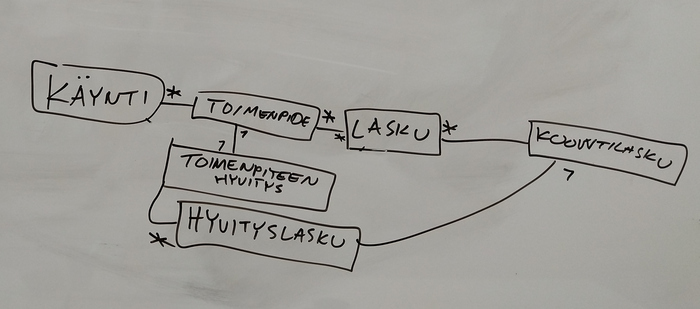
\includegraphics[width=\textwidth,height=0.3\textheight]{illustration/malli1.jpg}
\caption{\label{malli1}: Ensimmäinen malli}
\end{figure}

Oikeastaan käynnillä voi olla monta erillistä asiaa, ne ovat
laskutettavia toimenpiteitä. Palaverin lopuksi aikaansaatu kaavio on
kuvassa \ref{malli1}.

Tämä päätettiin toteuttaa.

Minulla meni torstaisen kokouksen jälkeen perjantai ja maanantai
perusrakenteen pystyttämiseen: Falcon, Ariadne GraphQL, Gunicorn ja
muutamia muita työkaluja. Lisäksi hommasin Pytest-testikirjaston, ja
opiskelin sen.

Lisäksi piti asentaa Apollo GraphQL-client ja Vue-cli, sekä plugin
Vue-Apollo.

Tiistaina sain ensimmäisen toiminnon, käyntien lisäämisen, valmiiksi.

Oli mielenkiintoista huomata, miten piirtämäni kuva ja tässä vaiheessa
aikaansaamani GraphQL-skeema muistuttivat läheisesti toisiaan.
GraphQL-queryjen sisältämät oliot rakensivat saman rakenteen, joka
tussitaululle piirsin. Sen sijaan GraphQL-mutaatioiden rooli ei ole
vielä auennut.

\hypertarget{viikko-2}{%
\section{Viikko 2}\label{viikko-2}}

Ensimmäisellä kehitykseen käyttämälläni viikolla (to-to) sain siis vain
ekan ominaisuuden valmiiksi. Sen jälkeen loppuviikosta tein vielä
käyntien laskutuksen. Lienee rehellistä arvioida, että noin viikon
kehitystyön myötä kaksi ``käyttäjätarinaa'' valmistui.

Perjantaina myös kirjoitin frontendia Vue-Apollolla ja käytin melkoisen
määrän aikaa kirjaston ominaisuuksien hahmottamiseen. Se ei kuulu
suoraan insinöörityön sisältöön, mutta toisaalta kuitenkin tarjoaa hyvän
kehyksen asioiden tekemiseen.

\hypertarget{viikko-3}{%
\section{Viikko 3}\label{viikko-3}}

Sain ensimmäisen version laskuhärvelistä valmiiksi. Tavoite oli Lauran
kanssa pitää asiasta palaveri perjantaina, mutta se peruuntui, koska
Laura oli tulossa kipeäksi.

Laskuhärveli toimii sinänsä, ja on hankala miettiä, onko siitä apua.

Kuitenkin domain-tason konseptien mallintaminen GraphQL-skeemaksi toimii
hyvin. Esimerkki, jossa koontilaskulla (ConsolidatedInvoice) voi olla
monta laskua (Invoice):

\begin{verbatim}
Type Invoice {
  number: Int
  sum: Float
  date: Date
}

type ConsolidatedInvoice {
  number: Int
  invoices: [Invoice]
}
\end{verbatim}

\hypertarget{palaveri-lauran-kanssa-tietomallin-kehittuxe4misestuxe4}{%
\section{27.9.2021 - Palaveri Lauran kanssa tietomallin
kehittämisestä}\label{palaveri-lauran-kanssa-tietomallin-kehittuxe4misestuxe4}}

Esittelin Lauralle tähän asti luomani softaproton. Pääasiallinen ongelma
on mielestäni laskun ja käynnin välisessä yhteydessä. Se, että laitetaan
käynti suoraan laskulle, on ongelmallista. Olin jo pitkin viikkoa
miettinyt, voisiko olla olemassa \textbf{Käyntirivi} ja \textbf{Käynnin
hyvitysrivi}, jotka sijaitsisivat laskulla ja koontilaskulla, ja
kumoaisivat toisensa.

Rupesin piirtämään Lauralle mallia, jossa Käynti liittyy Invoice-olioon,
ja Invoicea vastaa Credit Note, joka kumoaa Invoicella olevia käyntejä.
Piirsin Invoice- ja Credit note -olioiden sisään viivoja edustamaan
näitä käyntejä.

Laura totesi, että oikeastaan kirjanpidon kannalta täytyy täyttyä jokin
\textbf{Laskutusperuste}, jotta asia voidaan laskuttaa. Innostuin tästä
termistä, ja pyysin Lauraa jatkamaan. Laura sanoi, että laskutusperuste
on se, jonka pohjalta voidaan valita asioita laskutettavaksi. Asiat,
jotka täyttävät laskutusperusteen, mutta joihin ei liity laskua, voidaan
esimerkiksi listata laskuttamista varten. Pohjimmiltaan laskutusperuste
voi olla joko tavara tai palvelu, koska niitähän kaikki firmat myyvät.
Valitsimme laskutusperustetta kuvaamaan englanninkielisen termin
\textbf{BasisForInvoicing}. Palvelu on \textbf{Service}.

Ehdotin mallia, jossa \textbf{Appointment} voidaan viedä
\textbf{Invoicelle} \textbf{ServiceRow}-olioksi, jos täyttyy
BasisForInvoicing-ehto. Laura kurtisteli kulmiaan, eikä sanonut mitään.
Kysyin siis, eikö malli oikein miellytä, ja Laura totesi, että se
näyttää liian monimutkaiselta.

Pyyhin taulun puhtaaksi, ja kokeilimme uudestaan. Tein \textbf{Invoice}
-olion, jonka alle laitoin \textbf{ServiceRow} -nimisen olion. Invoicea
vastaamaan piirsin \textbf{CreditNote} -olion, jonka alle
\textbf{ServiceCreditRow}. Sivummas piirsin Appointment-olion, ja
pohdimme, mikä sen suhde voisi olla laskutukseen.

\begin{figure}
\centering
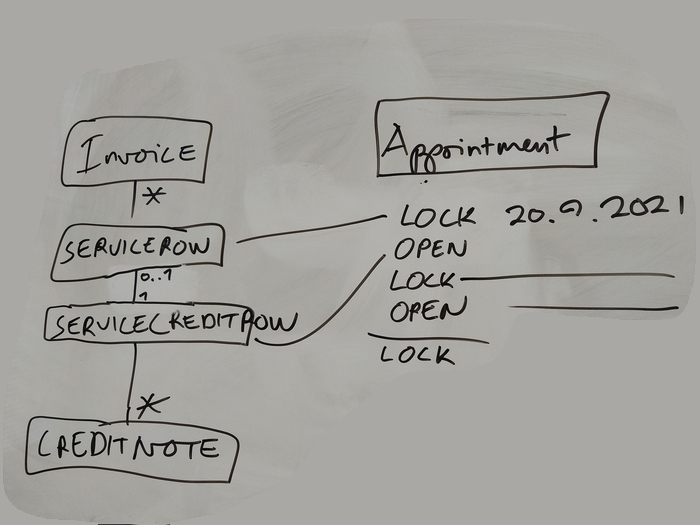
\includegraphics[width=\textwidth,height=0.5\textheight]{illustration/malli2.jpg}
\caption{\label{malli2}Toinen malli}
\end{figure}

Yhtäkkiä minulla välähti: mitä, jos tehtäisiin ikäänkuin loki
\textbf{Appointment}-olion sisälle: sinne tallennettaisiin
lukitustapahtuma, kun \textbf{Appointment} liitetään laskulle luomalla
sitä vastaava \textbf{ServiceRow}. Ja vastaavasti kun
\textbf{ServiceRow} hyvitettäisiin \textbf{ServiceCreditRown} avulla,
voitaisiin luoda avaustapahtuma. Näin ollen \textbf{Appointment}-luokan
alla olisi lista tapahtumia, ja listan avulla nähtäisiin sekä
laskutushistoria, että myös käynnin tämänhetkinen laskutustilanne:
Laskuttamatta vai avoinna? Esitän mallin kuvassa \ref{malli2}.

Laura huomautti, että tämä ei kuitenkaan ratkaise sitä pääongelmaa, joka
meillä on ollut: että käynnin hinta pitäisi jakaa monelle eri
maksajalle, joille lähetettyjä laskuja on voitava hyvittää itsenäisesti.

Niinpä pyyhin taas koko taulun puhtaaksi, ja lähdimme taas uudelleen
liikkeelle.

Nyt Käynnin alle lisättiin erillinen, laskutustarkoituksiin käytettävä
olio, jonka nimeksi pistettiin \textbf{BasisForInvoicing}. Tämä
BasisForInvoicing voidaan jakaa osiin, ja jokainen osa sisältää oman
erillisen listansa laskutustapahtumista: onko osa liitetty laskuun, vai
onko se hyvitetty ja taas siis avoinna.

\begin{figure}
\centering
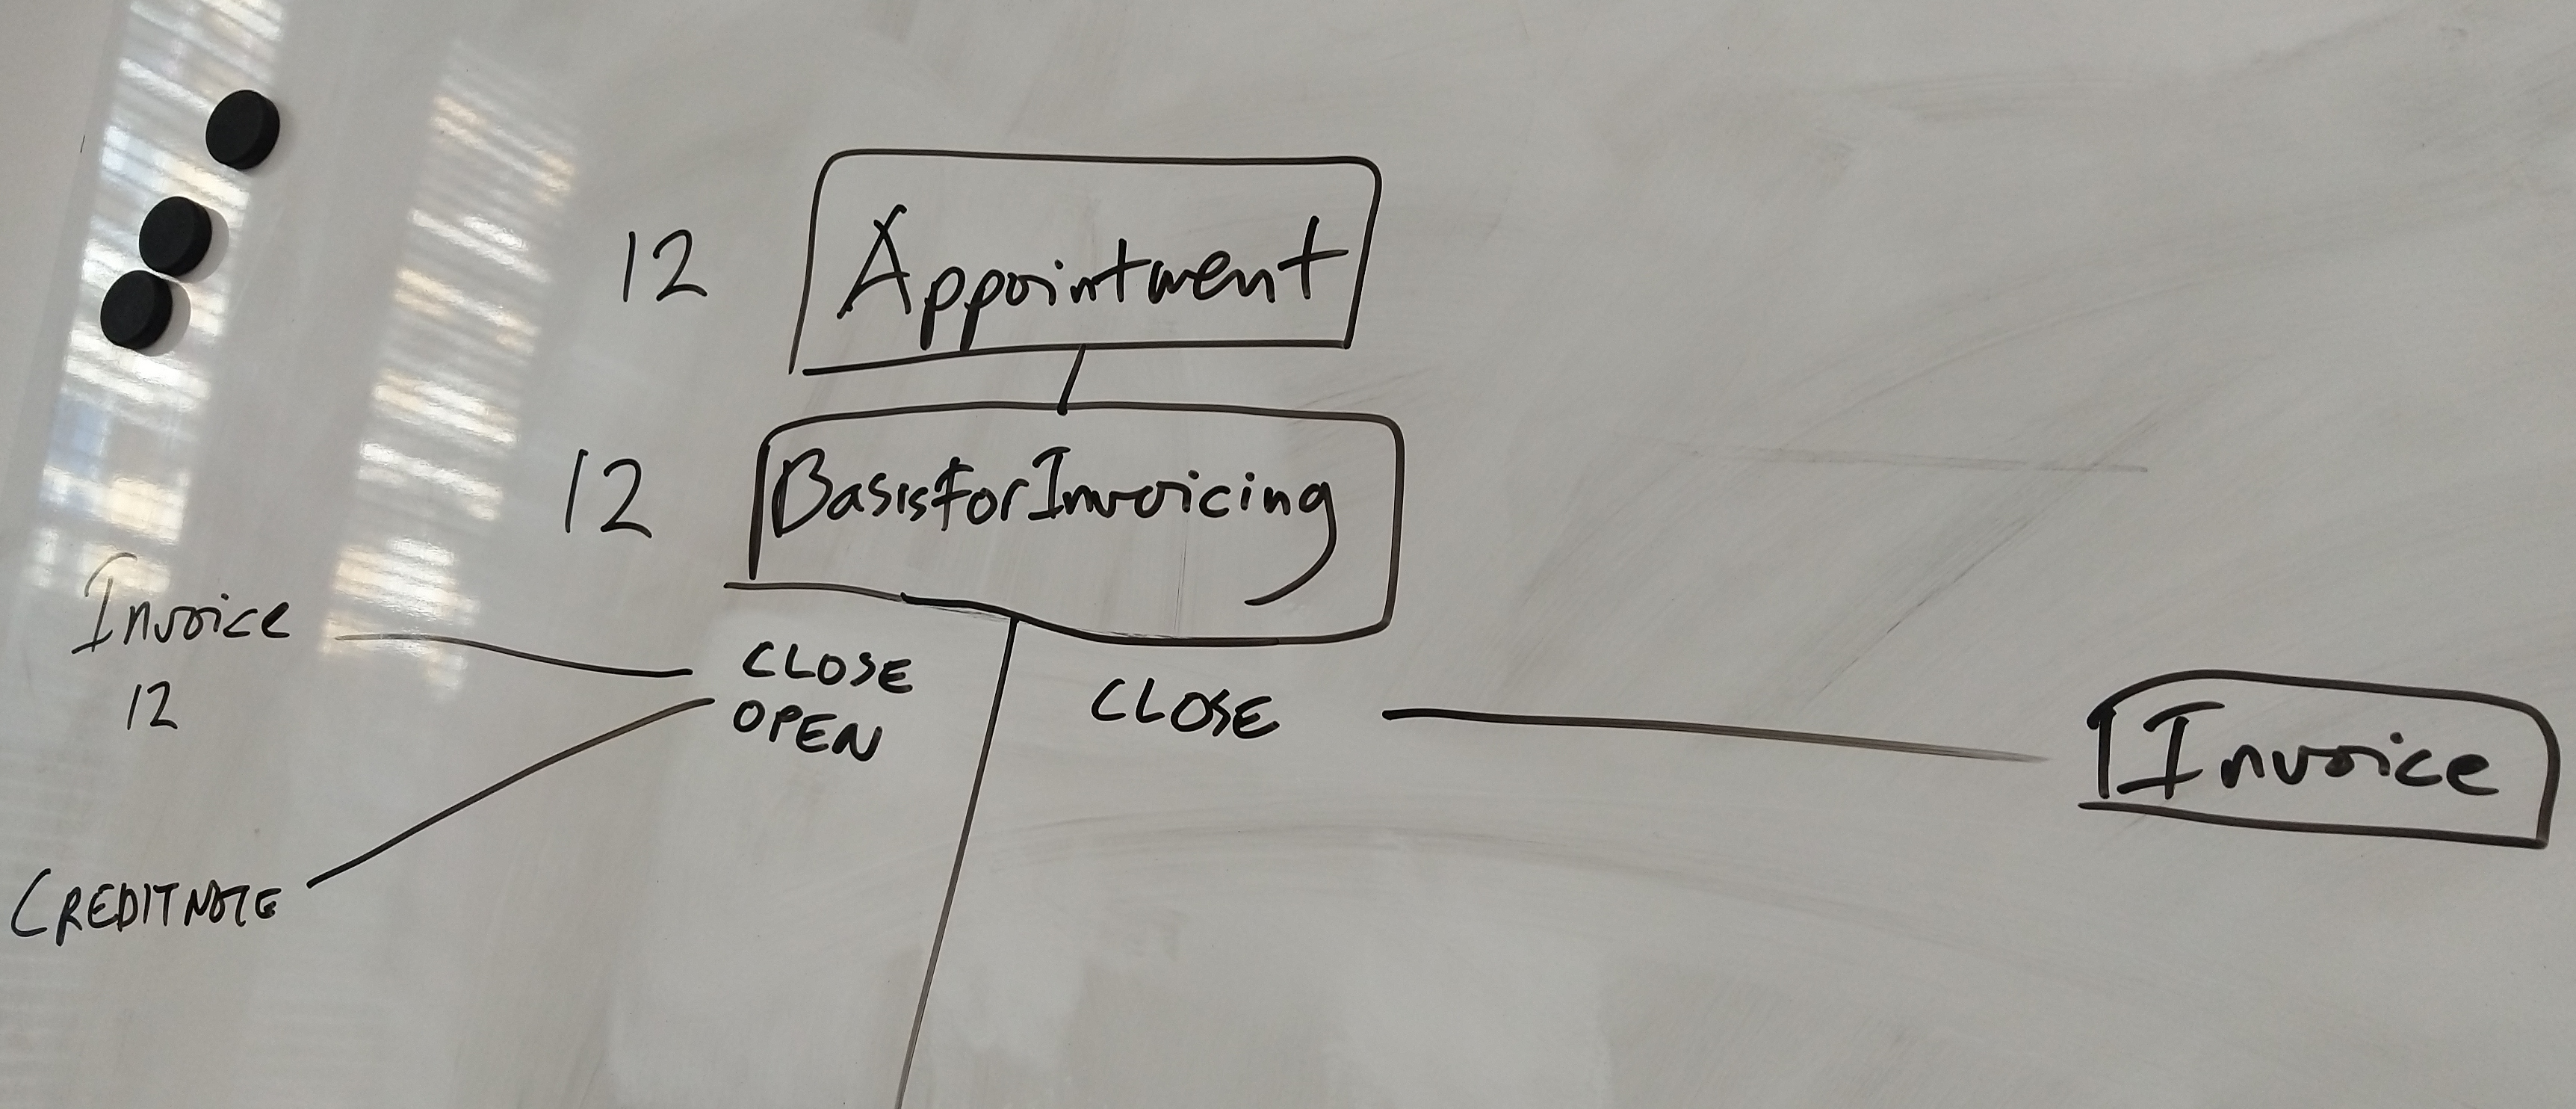
\includegraphics[width=\textwidth,height=0.5\textheight]{illustration/malli3.jpg}
\caption{\label{malli3}Kolmas malli}
\end{figure}

Tämä tuntui meistä hyvältä mallilta, ja sen pohjalta ryhdyin koodaamaan.
Tätä mallia esittää kuva \ref{malli3}. Sovittiin uusi palaveri viikon
päähän.
% Sample content to demonstrate appendix in LaTeX. You
% are safe to delete this lines (and the next samples) once you refreshed your LaTeX
% skills (and safe to delete the sample folder and all its file too).

%\addtocontents{toc}{\vspace{11pt}}%fix vertical space for Table of Content
% \liite{2}
% \input{sample/Xappendix2.tex}

% \addtocontents{toc}{\vspace{11pt}}
% \liite{3}
% \input{sample/X_R_example.tex}


%----------------------------------------------------------------------------------------
%	THIS IS THE END
%----------------------------------------------------------------------------------------
\end{document}
